%!TEX encoding = UTF-8 Unicode

\documentclass[landscape]{book}
\usepackage[a3paper]{geometry}

\usepackage{verbatim}

\usepackage{hyperref}

\usepackage{tikz}

\usetikzlibrary{
  arrows,
  shapes.misc,% wg. rounded rectangle
  shapes.arrows,%
  matrix,%
  scopes,%
  shadows%
}

\tikzset{
  nonterminal/.style={
    % The shape:
    rectangle,
    % The size:
    minimum size=6mm,
    % The border:
    very thick,
    draw=red!50!black!50,         % 50% red and 50% black,
                                  % and that mixed with 50% white
    % The filling:
    top color=white,              % a shading that is white at the top...
    bottom color=red!50!black!20, % and something else at the bottom
    % Font
    font=\itshape\small
  },
  terminal/.style={
    % The shape:
    rounded rectangle,
    minimum size=6mm,
    % The rest
    very thick,draw=black!50,
    top color=white,bottom color=black!20,
    font=\ttfamily\small
  },
  firstPoint/.style={circle,>=stealth',thick,draw=black!50},
  point/.style={coordinate,>=stealth',thick,draw=black!50},
  tip/.style={->,shorten >=0.007pt},
  lastPoint/.style={rectangle,>=stealth',thick,draw=black!50},
  every join/.style={rounded corners}
}

\newcommand\nonTerminalSection[2]{\section{Nonterminal \texttt{#1}}\label{nt:#2}}
\newcommand\ruleSubsection[3]{\subsection{Component \texttt{#1}, in file \texttt{#2}, line #3}}
\newcommand\ruleMatrixColumnSeparation{3mm}
\newcommand\ruleMatrixRowSeparation{3mm}
\newcommand\nonTerminalSymbol[2]{\hyperref[nt:#2]{#1}}
\newcommand\startSymbol[2]{The start symbol is \hyperref[nt:#2]{#1}.}

\newcommand\nonTerminalSummaryStart{This is the alphabetical list of non terminal : }
\newcommand\nonTerminalSummary[2]{\hyperref[nt:#2]{#1}}
\newcommand\nonTerminalSummarySeparator{, }
\newcommand\nonTerminalSummaryEnd{.\\}

\begin{document}

\title{\Huge{Grammar \texttt{arxmlmetaparser\_grammar}}}
\date \today 

\maketitle

\startSymbol{arxmlmetaparser\_start\_symbol}{0}

\nonTerminalSummaryStart \nonTerminalSummary{arxmlmetaparser\_start\_symbol}{0}\nonTerminalSummarySeparator \nonTerminalSummary{xml\_header}{1}\nonTerminalSummarySeparator \nonTerminalSummary{xsd\_annotation}{2}\nonTerminalSummarySeparator \nonTerminalSummary{xsd\_appinfo}{3}\nonTerminalSummarySeparator \nonTerminalSummary{xsd\_attribute}{4}\nonTerminalSummarySeparator \nonTerminalSummary{xsd\_attributeGroup}{5}\nonTerminalSummarySeparator \nonTerminalSummary{xsd\_choice}{6}\nonTerminalSummarySeparator \nonTerminalSummary{xsd\_complexType}{7}\nonTerminalSummarySeparator \nonTerminalSummary{xsd\_documentation}{8}\nonTerminalSummarySeparator \nonTerminalSummary{xsd\_element}{9}\nonTerminalSummarySeparator \nonTerminalSummary{xsd\_enumeration}{10}\nonTerminalSummarySeparator \nonTerminalSummary{xsd\_extension}{11}\nonTerminalSummarySeparator \nonTerminalSummary{xsd\_group}{12}\nonTerminalSummarySeparator \nonTerminalSummary{xsd\_ignore\_attributes}{22}\nonTerminalSummarySeparator \nonTerminalSummary{xsd\_import}{13}\nonTerminalSummarySeparator \nonTerminalSummary{xsd\_maxLength}{19}\nonTerminalSummarySeparator \nonTerminalSummary{xsd\_pattern}{20}\nonTerminalSummarySeparator \nonTerminalSummary{xsd\_restriction}{14}\nonTerminalSummarySeparator \nonTerminalSummary{xsd\_schema}{15}\nonTerminalSummarySeparator \nonTerminalSummary{xsd\_sequence}{16}\nonTerminalSummarySeparator \nonTerminalSummary{xsd\_simpleContent}{17}\nonTerminalSummarySeparator \nonTerminalSummary{xsd\_simpleType}{18}\nonTerminalSummarySeparator \nonTerminalSummary{xsd\_whiteSpace}{21}\nonTerminalSummaryEnd \nonTerminalSection{arxmlmetaparser\_start\_symbol}{0}

\ruleSubsection{arxmlmetaparser\_syntax}{arxmlmetaparser\_syntax}{31}

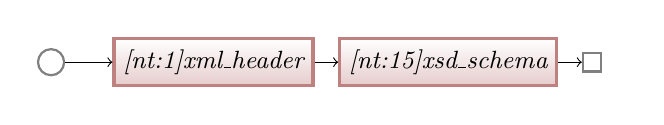
\begin{tikzpicture}
  \matrix[column sep=\ruleMatrixColumnSeparation, row sep=\ruleMatrixRowSeparation] {
    \node (P0start) [firstPoint] {}; & & \node (p0-2) [nonterminal] {\nonTerminalSymbol{xml\_header}{1}}; & \node (p0-3) [nonterminal] {\nonTerminalSymbol{xsd\_schema}{15}}; & \node (p0-4) [lastPoint] {}; & \\
  };
  \draw[->] (P0start) -- (p0-2) ;
  \draw[->] (p0-2) -- (p0-3) ;
  \draw[->] (p0-3) -- (p0-4) ;
\end{tikzpicture}

\nonTerminalSection{xml\_header}{1}

\ruleSubsection{arxmlmetaparser\_syntax}{arxmlmetaparser\_syntax}{61}

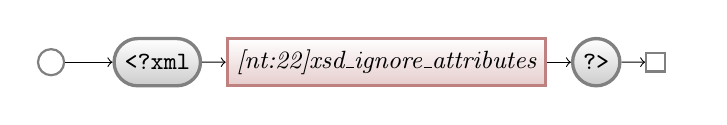
\begin{tikzpicture}
  \matrix[column sep=\ruleMatrixColumnSeparation, row sep=\ruleMatrixRowSeparation] {
    \node (P0start) [firstPoint] {}; & & \node (p0-2) [terminal] {<?xml}; & \node (p0-3) [nonterminal] {\nonTerminalSymbol{xsd\_ignore\_attributes}{22}}; & \node (p0-4) [terminal] {?>}; & \node (p0-5) [lastPoint] {}; & \\
  };
  \draw[->] (P0start) -- (p0-2) ;
  \draw[->] (p0-2) -- (p0-3) ;
  \draw[->] (p0-3) -- (p0-4) ;
  \draw[->] (p0-4) -- (p0-5) ;
\end{tikzpicture}

\nonTerminalSection{xsd\_annotation}{2}

\ruleSubsection{arxmlmetaparser\_syntax}{arxmlmetaparser\_syntax}{75}

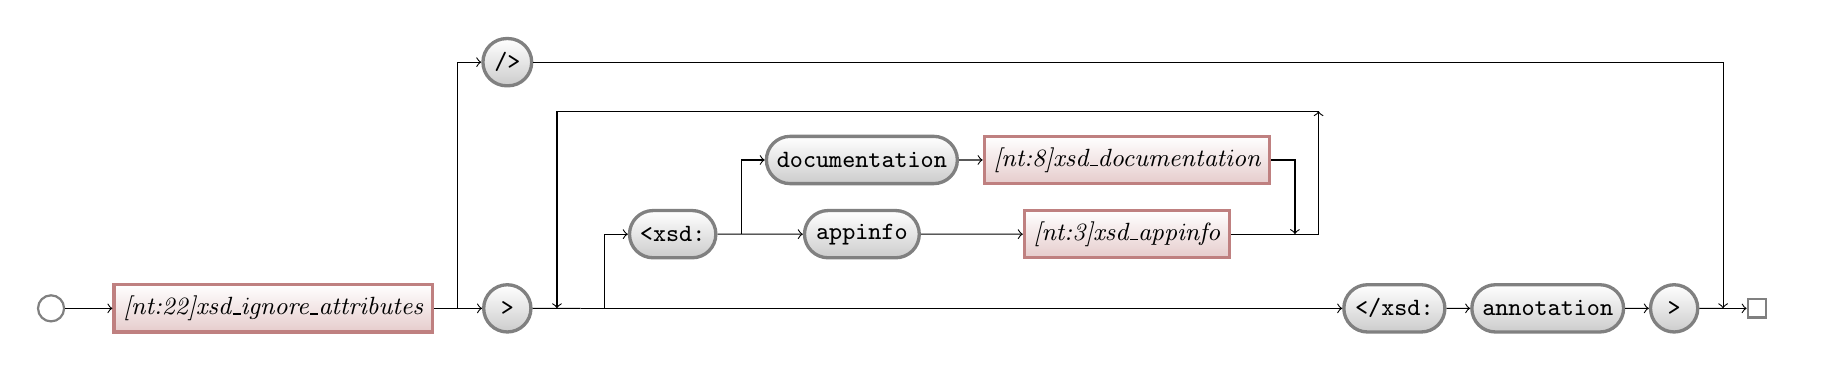
\begin{tikzpicture}
  \matrix[column sep=\ruleMatrixColumnSeparation, row sep=\ruleMatrixRowSeparation] {
    & & & & \node (p4-4) [terminal] {/>}; & \\
    & & & & & & & & & & & & & \node (p3-13) [point] {}; & \\
    & & & & & & & & & & \node (p2-10) [terminal] {documentation}; & \node (p2-11) [nonterminal] {\nonTerminalSymbol{xsd\_documentation}{8}}; & \\
    & & & & & & & & \node (p1-8) [terminal] {<xsd:}; & \node (p1-9) [point] {}; & \node (p1-10) [terminal] {appinfo}; & \node (p1-11) [nonterminal] {\nonTerminalSymbol{xsd\_appinfo}{3}}; & \node (p1-12) [point] {}; & \\
    \node (P0start) [firstPoint] {}; & & \node (p0-2) [nonterminal] {\nonTerminalSymbol{xsd\_ignore\_attributes}{22}}; & \node (p0-3) [point] {}; & \node (p0-4) [terminal] {>}; & \node (p0-5) [point] {}; & \node (p0-6) [point] {}; & \node (p0-7) [point] {}; & & & & & & & \node (p0-14) [terminal] {</xsd:}; & \node (p0-15) [terminal] {annotation}; & \node (p0-16) [terminal] {>}; & \node (p0-17) [point] {}; & \node (p0-18) [lastPoint] {}; & \\
  };
  \draw[->] (P0start) -- (p0-2) ;
  \draw[->] (p0-2) -- (p0-4) ;
  \draw (p0-4) -- (p0-6) ;
  \draw[->] (p0-7) |- (p1-8) ;
  \draw[->] (p1-8) -- (p1-10) ;
  \draw[->] (p1-10) -- (p1-11) ;
  \draw[->] (p1-9) |- (p2-10) ;
  \draw[->] (p2-10) -- (p2-11) ;
  \draw (p1-11) -- (p1-12) ;
  \draw[->] (p2-11) -| (p1-12) ;
  \draw[->] (p3-13) -| (p0-5) ;
  \draw[->] (p1-12) -| (p3-13) ;
  \draw[->] (p0-6) -- (p0-14) ;
  \draw[->] (p0-14) -- (p0-15) ;
  \draw[->] (p0-15) -- (p0-16) ;
  \draw[->] (p0-3) |- (p4-4) ;
  \draw (p0-16) -- (p0-17) ;
  \draw[->] (p4-4) -| (p0-17) ;
  \draw[->] (p0-17) -- (p0-18) ;
\end{tikzpicture}

\nonTerminalSection{xsd\_appinfo}{3}

\ruleSubsection{arxmlmetaparser\_syntax}{arxmlmetaparser\_syntax}{101}

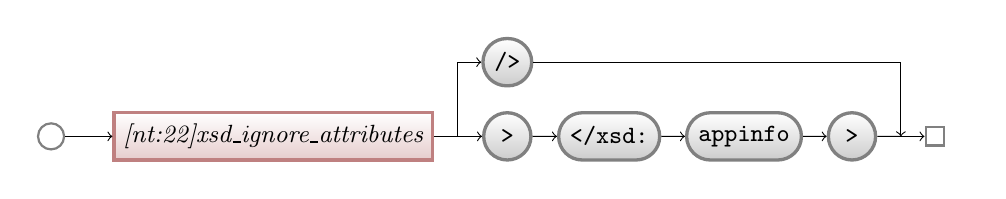
\begin{tikzpicture}
  \matrix[column sep=\ruleMatrixColumnSeparation, row sep=\ruleMatrixRowSeparation] {
    & & & & \node (p1-4) [terminal] {/>}; & \\
    \node (P0start) [firstPoint] {}; & & \node (p0-2) [nonterminal] {\nonTerminalSymbol{xsd\_ignore\_attributes}{22}}; & \node (p0-3) [point] {}; & \node (p0-4) [terminal] {>}; & \node (p0-5) [terminal] {</xsd:}; & \node (p0-6) [terminal] {appinfo}; & \node (p0-7) [terminal] {>}; & \node (p0-8) [point] {}; & \node (p0-9) [lastPoint] {}; & \\
  };
  \draw[->] (P0start) -- (p0-2) ;
  \draw[->] (p0-2) -- (p0-4) ;
  \draw[->] (p0-4) -- (p0-5) ;
  \draw[->] (p0-5) -- (p0-6) ;
  \draw[->] (p0-6) -- (p0-7) ;
  \draw[->] (p0-3) |- (p1-4) ;
  \draw (p0-7) -- (p0-8) ;
  \draw[->] (p1-4) -| (p0-8) ;
  \draw[->] (p0-8) -- (p0-9) ;
\end{tikzpicture}

\nonTerminalSection{xsd\_attribute}{4}

\ruleSubsection{arxmlmetaparser\_syntax}{arxmlmetaparser\_syntax}{118}

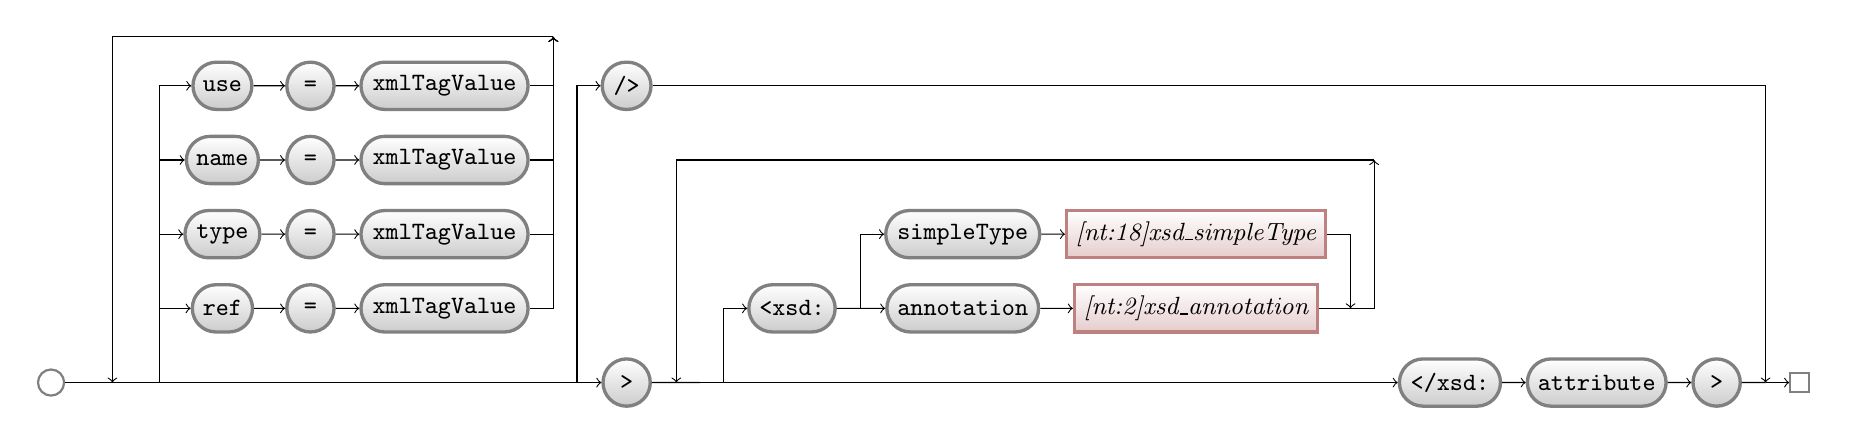
\begin{tikzpicture}
  \matrix[column sep=\ruleMatrixColumnSeparation, row sep=\ruleMatrixRowSeparation] {
    & & & & & & & & \node (p5-8) [point] {}; & \\
    & & & & & \node (p4-5) [terminal] {use}; & \node (p4-6) [terminal] {=}; & \node (p4-7) [terminal] {xmlTagValue}; & & & \node (p4-10) [terminal] {/>}; & \\
    & & & & & \node (p3-5) [terminal] {name}; & \node (p3-6) [terminal] {=}; & \node (p3-7) [terminal] {xmlTagValue}; & & & & & & & & & & & & \node (p3-19) [point] {}; & \\
    & & & & & \node (p2-5) [terminal] {type}; & \node (p2-6) [terminal] {=}; & \node (p2-7) [terminal] {xmlTagValue}; & & & & & & & & & \node (p2-16) [terminal] {simpleType}; & \node (p2-17) [nonterminal] {\nonTerminalSymbol{xsd\_simpleType}{18}}; & \\
    & & & & & \node (p1-5) [terminal] {ref}; & \node (p1-6) [terminal] {=}; & \node (p1-7) [terminal] {xmlTagValue}; & & & & & & & \node (p1-14) [terminal] {<xsd:}; & \node (p1-15) [point] {}; & \node (p1-16) [terminal] {annotation}; & \node (p1-17) [nonterminal] {\nonTerminalSymbol{xsd\_annotation}{2}}; & \node (p1-18) [point] {}; & \\
    \node (P0start) [firstPoint] {}; & & \node (p0-2) [point] {}; & \node (p0-3) [point] {}; & \node (p0-4) [point] {}; & & & & & \node (p0-9) [point] {}; & \node (p0-10) [terminal] {>}; & \node (p0-11) [point] {}; & \node (p0-12) [point] {}; & \node (p0-13) [point] {}; & & & & & & & \node (p0-20) [terminal] {</xsd:}; & \node (p0-21) [terminal] {attribute}; & \node (p0-22) [terminal] {>}; & \node (p0-23) [point] {}; & \node (p0-24) [lastPoint] {}; & \\
  };
  \draw (P0start) -- (p0-3) ;
  \draw[->] (p0-4) |- (p1-5) ;
  \draw[->] (p1-5) -- (p1-6) ;
  \draw[->] (p1-6) -- (p1-7) ;
  \draw[->] (p0-4) |- (p2-5) ;
  \draw[->] (p2-5) -- (p2-6) ;
  \draw[->] (p2-6) -- (p2-7) ;
  \draw[->] (p0-4) |- (p3-5) ;
  \draw[->] (p3-5) -- (p3-6) ;
  \draw[->] (p3-6) -- (p3-7) ;
  \draw[->] (p0-4) |- (p4-5) ;
  \draw[->] (p4-5) -- (p4-6) ;
  \draw[->] (p4-6) -- (p4-7) ;
  \draw[->] (p5-8) -| (p0-2) ;
  \draw[->] (p1-7) -| (p5-8) ;
  \draw[->] (p2-7) -| (p5-8) ;
  \draw[->] (p3-7) -| (p5-8) ;
  \draw[->] (p4-7) -| (p5-8) ;
  \draw[->] (p0-3) -- (p0-10) ;
  \draw (p0-10) -- (p0-12) ;
  \draw[->] (p0-13) |- (p1-14) ;
  \draw[->] (p1-14) -- (p1-16) ;
  \draw[->] (p1-16) -- (p1-17) ;
  \draw[->] (p1-15) |- (p2-16) ;
  \draw[->] (p2-16) -- (p2-17) ;
  \draw (p1-17) -- (p1-18) ;
  \draw[->] (p2-17) -| (p1-18) ;
  \draw[->] (p3-19) -| (p0-11) ;
  \draw[->] (p1-18) -| (p3-19) ;
  \draw[->] (p0-12) -- (p0-20) ;
  \draw[->] (p0-20) -- (p0-21) ;
  \draw[->] (p0-21) -- (p0-22) ;
  \draw[->] (p0-9) |- (p4-10) ;
  \draw (p0-22) -- (p0-23) ;
  \draw[->] (p4-10) -| (p0-23) ;
  \draw[->] (p0-23) -- (p0-24) ;
\end{tikzpicture}

\nonTerminalSection{xsd\_attributeGroup}{5}

\ruleSubsection{arxmlmetaparser\_syntax}{arxmlmetaparser\_syntax}{191}

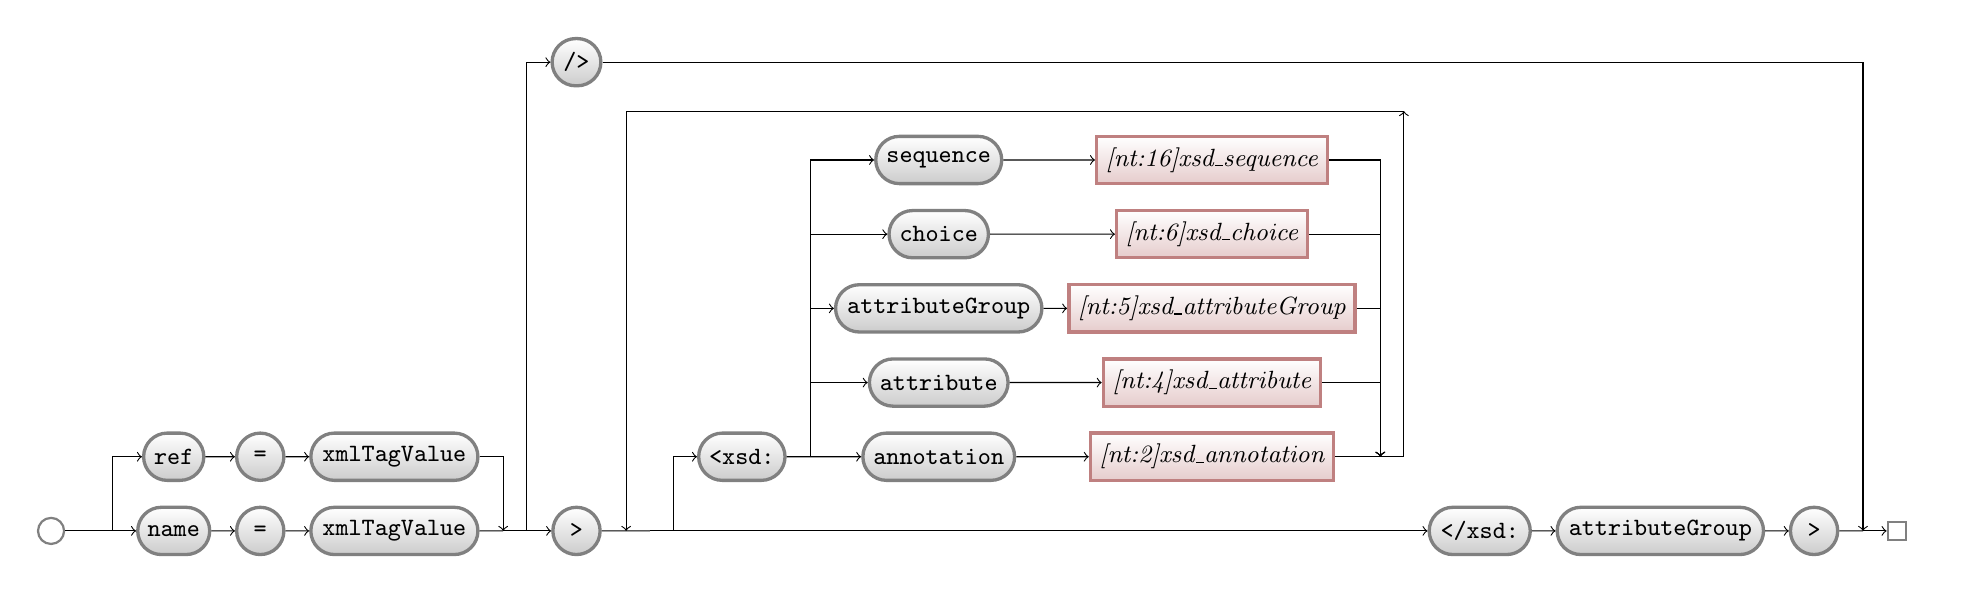
\begin{tikzpicture}
  \matrix[column sep=\ruleMatrixColumnSeparation, row sep=\ruleMatrixRowSeparation] {
    & & & & & & & & \node (p7-8) [terminal] {/>}; & \\
    & & & & & & & & & & & & & & & & & \node (p6-17) [point] {}; & \\
    & & & & & & & & & & & & & & \node (p5-14) [terminal] {sequence}; & \node (p5-15) [nonterminal] {\nonTerminalSymbol{xsd\_sequence}{16}}; & \\
    & & & & & & & & & & & & & & \node (p4-14) [terminal] {choice}; & \node (p4-15) [nonterminal] {\nonTerminalSymbol{xsd\_choice}{6}}; & \\
    & & & & & & & & & & & & & & \node (p3-14) [terminal] {attributeGroup}; & \node (p3-15) [nonterminal] {\nonTerminalSymbol{xsd\_attributeGroup}{5}}; & \\
    & & & & & & & & & & & & & & \node (p2-14) [terminal] {attribute}; & \node (p2-15) [nonterminal] {\nonTerminalSymbol{xsd\_attribute}{4}}; & \\
    & & & \node (p1-3) [terminal] {ref}; & \node (p1-4) [terminal] {=}; & \node (p1-5) [terminal] {xmlTagValue}; & & & & & & & \node (p1-12) [terminal] {<xsd:}; & \node (p1-13) [point] {}; & \node (p1-14) [terminal] {annotation}; & \node (p1-15) [nonterminal] {\nonTerminalSymbol{xsd\_annotation}{2}}; & \node (p1-16) [point] {}; & \\
    \node (P0start) [firstPoint] {}; & & \node (p0-2) [point] {}; & \node (p0-3) [terminal] {name}; & \node (p0-4) [terminal] {=}; & \node (p0-5) [terminal] {xmlTagValue}; & \node (p0-6) [point] {}; & \node (p0-7) [point] {}; & \node (p0-8) [terminal] {>}; & \node (p0-9) [point] {}; & \node (p0-10) [point] {}; & \node (p0-11) [point] {}; & & & & & & & \node (p0-18) [terminal] {</xsd:}; & \node (p0-19) [terminal] {attributeGroup}; & \node (p0-20) [terminal] {>}; & \node (p0-21) [point] {}; & \node (p0-22) [lastPoint] {}; & \\
  };
  \draw[->] (P0start) -- (p0-3) ;
  \draw[->] (p0-3) -- (p0-4) ;
  \draw[->] (p0-4) -- (p0-5) ;
  \draw[->] (p0-2) |- (p1-3) ;
  \draw[->] (p1-3) -- (p1-4) ;
  \draw[->] (p1-4) -- (p1-5) ;
  \draw (p0-5) -- (p0-6) ;
  \draw[->] (p1-5) -| (p0-6) ;
  \draw[->] (p0-6) -- (p0-8) ;
  \draw (p0-8) -- (p0-10) ;
  \draw[->] (p0-11) |- (p1-12) ;
  \draw[->] (p1-12) -- (p1-14) ;
  \draw[->] (p1-14) -- (p1-15) ;
  \draw[->] (p1-13) |- (p2-14) ;
  \draw[->] (p2-14) -- (p2-15) ;
  \draw[->] (p1-13) |- (p3-14) ;
  \draw[->] (p3-14) -- (p3-15) ;
  \draw[->] (p1-13) |- (p4-14) ;
  \draw[->] (p4-14) -- (p4-15) ;
  \draw[->] (p1-13) |- (p5-14) ;
  \draw[->] (p5-14) -- (p5-15) ;
  \draw (p1-15) -- (p1-16) ;
  \draw[->] (p2-15) -| (p1-16) ;
  \draw[->] (p3-15) -| (p1-16) ;
  \draw[->] (p4-15) -| (p1-16) ;
  \draw[->] (p5-15) -| (p1-16) ;
  \draw[->] (p6-17) -| (p0-9) ;
  \draw[->] (p1-16) -| (p6-17) ;
  \draw[->] (p0-10) -- (p0-18) ;
  \draw[->] (p0-18) -- (p0-19) ;
  \draw[->] (p0-19) -- (p0-20) ;
  \draw[->] (p0-7) |- (p7-8) ;
  \draw (p0-20) -- (p0-21) ;
  \draw[->] (p7-8) -| (p0-21) ;
  \draw[->] (p0-21) -- (p0-22) ;
\end{tikzpicture}

\nonTerminalSection{xsd\_choice}{6}

\ruleSubsection{arxmlmetaparser\_syntax}{arxmlmetaparser\_syntax}{265}

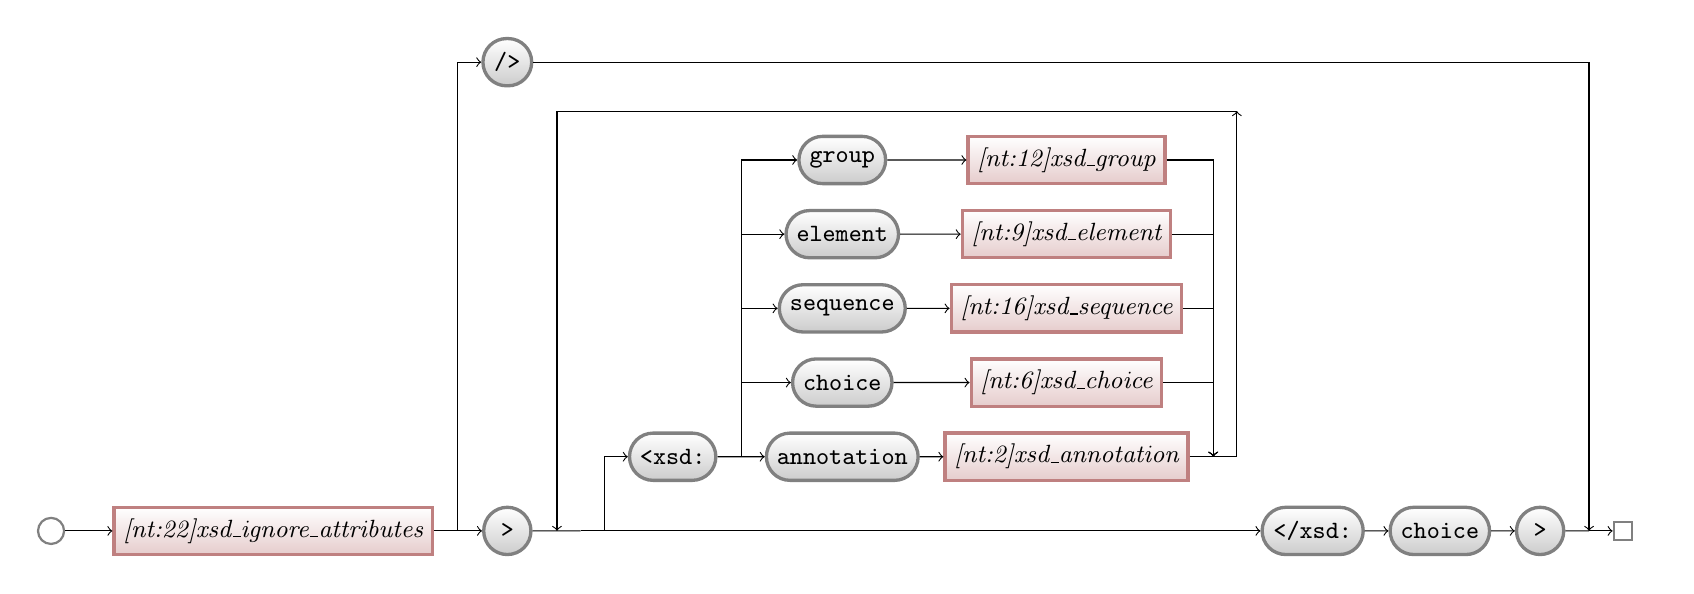
\begin{tikzpicture}
  \matrix[column sep=\ruleMatrixColumnSeparation, row sep=\ruleMatrixRowSeparation] {
    & & & & \node (p7-4) [terminal] {/>}; & \\
    & & & & & & & & & & & & & \node (p6-13) [point] {}; & \\
    & & & & & & & & & & \node (p5-10) [terminal] {group}; & \node (p5-11) [nonterminal] {\nonTerminalSymbol{xsd\_group}{12}}; & \\
    & & & & & & & & & & \node (p4-10) [terminal] {element}; & \node (p4-11) [nonterminal] {\nonTerminalSymbol{xsd\_element}{9}}; & \\
    & & & & & & & & & & \node (p3-10) [terminal] {sequence}; & \node (p3-11) [nonterminal] {\nonTerminalSymbol{xsd\_sequence}{16}}; & \\
    & & & & & & & & & & \node (p2-10) [terminal] {choice}; & \node (p2-11) [nonterminal] {\nonTerminalSymbol{xsd\_choice}{6}}; & \\
    & & & & & & & & \node (p1-8) [terminal] {<xsd:}; & \node (p1-9) [point] {}; & \node (p1-10) [terminal] {annotation}; & \node (p1-11) [nonterminal] {\nonTerminalSymbol{xsd\_annotation}{2}}; & \node (p1-12) [point] {}; & \\
    \node (P0start) [firstPoint] {}; & & \node (p0-2) [nonterminal] {\nonTerminalSymbol{xsd\_ignore\_attributes}{22}}; & \node (p0-3) [point] {}; & \node (p0-4) [terminal] {>}; & \node (p0-5) [point] {}; & \node (p0-6) [point] {}; & \node (p0-7) [point] {}; & & & & & & & \node (p0-14) [terminal] {</xsd:}; & \node (p0-15) [terminal] {choice}; & \node (p0-16) [terminal] {>}; & \node (p0-17) [point] {}; & \node (p0-18) [lastPoint] {}; & \\
  };
  \draw[->] (P0start) -- (p0-2) ;
  \draw[->] (p0-2) -- (p0-4) ;
  \draw (p0-4) -- (p0-6) ;
  \draw[->] (p0-7) |- (p1-8) ;
  \draw[->] (p1-8) -- (p1-10) ;
  \draw[->] (p1-10) -- (p1-11) ;
  \draw[->] (p1-9) |- (p2-10) ;
  \draw[->] (p2-10) -- (p2-11) ;
  \draw[->] (p1-9) |- (p3-10) ;
  \draw[->] (p3-10) -- (p3-11) ;
  \draw[->] (p1-9) |- (p4-10) ;
  \draw[->] (p4-10) -- (p4-11) ;
  \draw[->] (p1-9) |- (p5-10) ;
  \draw[->] (p5-10) -- (p5-11) ;
  \draw (p1-11) -- (p1-12) ;
  \draw[->] (p2-11) -| (p1-12) ;
  \draw[->] (p3-11) -| (p1-12) ;
  \draw[->] (p4-11) -| (p1-12) ;
  \draw[->] (p5-11) -| (p1-12) ;
  \draw[->] (p6-13) -| (p0-5) ;
  \draw[->] (p1-12) -| (p6-13) ;
  \draw[->] (p0-6) -- (p0-14) ;
  \draw[->] (p0-14) -- (p0-15) ;
  \draw[->] (p0-15) -- (p0-16) ;
  \draw[->] (p0-3) |- (p7-4) ;
  \draw (p0-16) -- (p0-17) ;
  \draw[->] (p7-4) -| (p0-17) ;
  \draw[->] (p0-17) -- (p0-18) ;
\end{tikzpicture}

\nonTerminalSection{xsd\_complexType}{7}

\ruleSubsection{arxmlmetaparser\_syntax}{arxmlmetaparser\_syntax}{297}

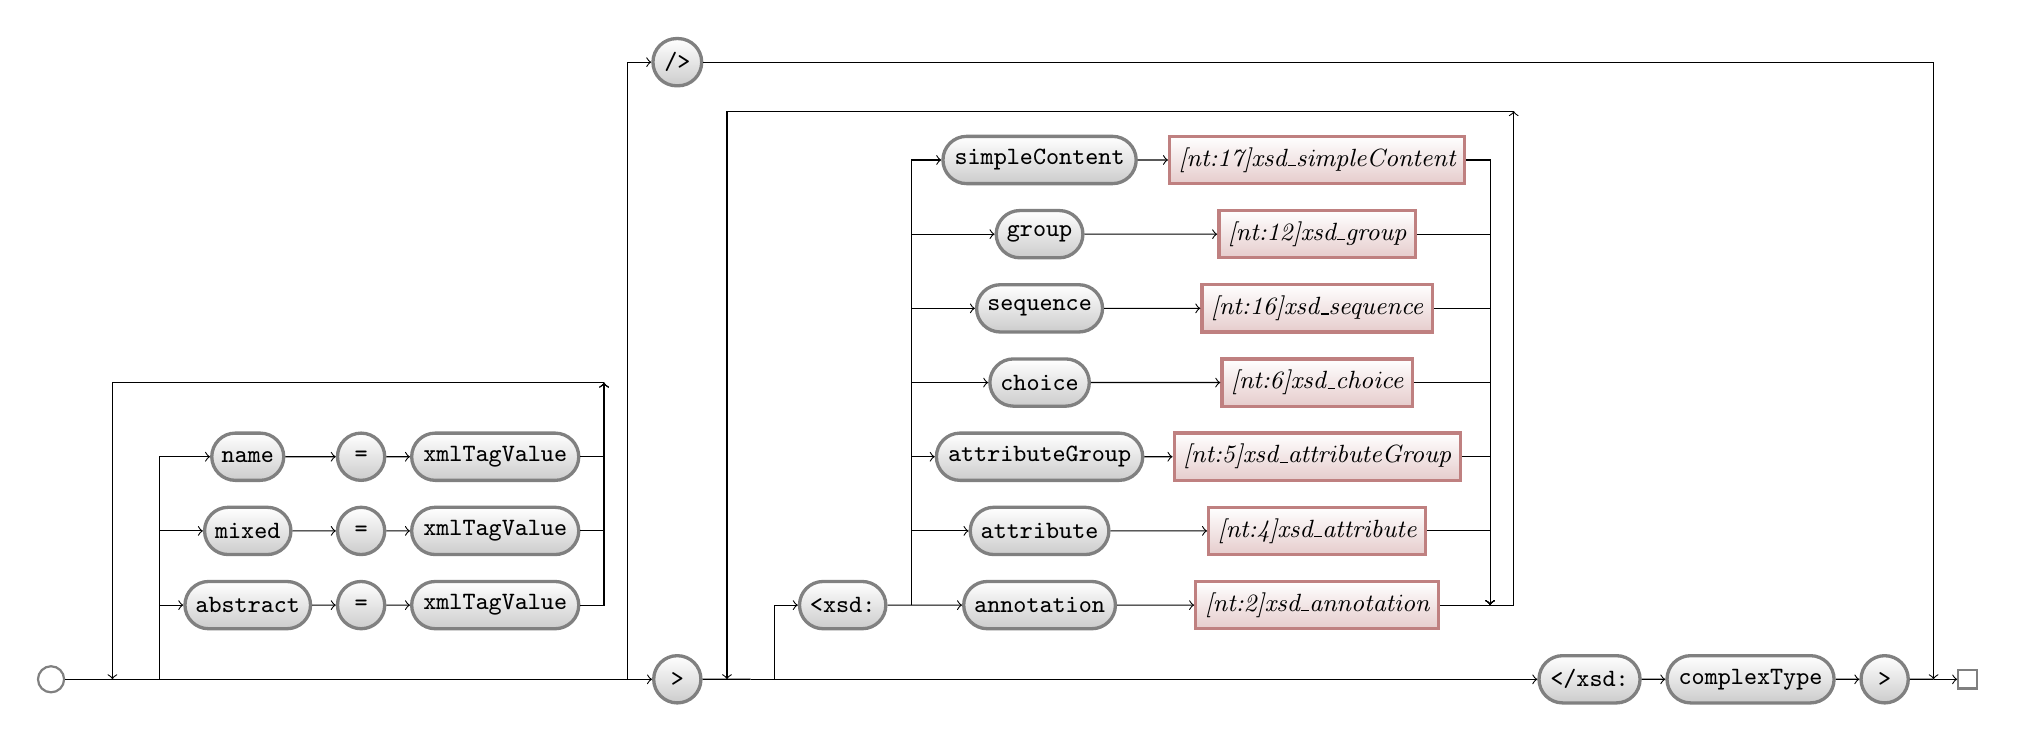
\begin{tikzpicture}
  \matrix[column sep=\ruleMatrixColumnSeparation, row sep=\ruleMatrixRowSeparation] {
    & & & & & & & & & & \node (p9-10) [terminal] {/>}; & \\
    & & & & & & & & & & & & & & & & & & & \node (p8-19) [point] {}; & \\
    & & & & & & & & & & & & & & & & \node (p7-16) [terminal] {simpleContent}; & \node (p7-17) [nonterminal] {\nonTerminalSymbol{xsd\_simpleContent}{17}}; & \\
    & & & & & & & & & & & & & & & & \node (p6-16) [terminal] {group}; & \node (p6-17) [nonterminal] {\nonTerminalSymbol{xsd\_group}{12}}; & \\
    & & & & & & & & & & & & & & & & \node (p5-16) [terminal] {sequence}; & \node (p5-17) [nonterminal] {\nonTerminalSymbol{xsd\_sequence}{16}}; & \\
    & & & & & & & & \node (p4-8) [point] {}; & & & & & & & & \node (p4-16) [terminal] {choice}; & \node (p4-17) [nonterminal] {\nonTerminalSymbol{xsd\_choice}{6}}; & \\
    & & & & & \node (p3-5) [terminal] {name}; & \node (p3-6) [terminal] {=}; & \node (p3-7) [terminal] {xmlTagValue}; & & & & & & & & & \node (p3-16) [terminal] {attributeGroup}; & \node (p3-17) [nonterminal] {\nonTerminalSymbol{xsd\_attributeGroup}{5}}; & \\
    & & & & & \node (p2-5) [terminal] {mixed}; & \node (p2-6) [terminal] {=}; & \node (p2-7) [terminal] {xmlTagValue}; & & & & & & & & & \node (p2-16) [terminal] {attribute}; & \node (p2-17) [nonterminal] {\nonTerminalSymbol{xsd\_attribute}{4}}; & \\
    & & & & & \node (p1-5) [terminal] {abstract}; & \node (p1-6) [terminal] {=}; & \node (p1-7) [terminal] {xmlTagValue}; & & & & & & & \node (p1-14) [terminal] {<xsd:}; & \node (p1-15) [point] {}; & \node (p1-16) [terminal] {annotation}; & \node (p1-17) [nonterminal] {\nonTerminalSymbol{xsd\_annotation}{2}}; & \node (p1-18) [point] {}; & \\
    \node (P0start) [firstPoint] {}; & & \node (p0-2) [point] {}; & \node (p0-3) [point] {}; & \node (p0-4) [point] {}; & & & & & \node (p0-9) [point] {}; & \node (p0-10) [terminal] {>}; & \node (p0-11) [point] {}; & \node (p0-12) [point] {}; & \node (p0-13) [point] {}; & & & & & & & \node (p0-20) [terminal] {</xsd:}; & \node (p0-21) [terminal] {complexType}; & \node (p0-22) [terminal] {>}; & \node (p0-23) [point] {}; & \node (p0-24) [lastPoint] {}; & \\
  };
  \draw (P0start) -- (p0-3) ;
  \draw[->] (p0-4) |- (p1-5) ;
  \draw[->] (p1-5) -- (p1-6) ;
  \draw[->] (p1-6) -- (p1-7) ;
  \draw[->] (p0-4) |- (p2-5) ;
  \draw[->] (p2-5) -- (p2-6) ;
  \draw[->] (p2-6) -- (p2-7) ;
  \draw[->] (p0-4) |- (p3-5) ;
  \draw[->] (p3-5) -- (p3-6) ;
  \draw[->] (p3-6) -- (p3-7) ;
  \draw[->] (p4-8) -| (p0-2) ;
  \draw[->] (p1-7) -| (p4-8) ;
  \draw[->] (p2-7) -| (p4-8) ;
  \draw[->] (p3-7) -| (p4-8) ;
  \draw[->] (p0-3) -- (p0-10) ;
  \draw (p0-10) -- (p0-12) ;
  \draw[->] (p0-13) |- (p1-14) ;
  \draw[->] (p1-14) -- (p1-16) ;
  \draw[->] (p1-16) -- (p1-17) ;
  \draw[->] (p1-15) |- (p2-16) ;
  \draw[->] (p2-16) -- (p2-17) ;
  \draw[->] (p1-15) |- (p3-16) ;
  \draw[->] (p3-16) -- (p3-17) ;
  \draw[->] (p1-15) |- (p4-16) ;
  \draw[->] (p4-16) -- (p4-17) ;
  \draw[->] (p1-15) |- (p5-16) ;
  \draw[->] (p5-16) -- (p5-17) ;
  \draw[->] (p1-15) |- (p6-16) ;
  \draw[->] (p6-16) -- (p6-17) ;
  \draw[->] (p1-15) |- (p7-16) ;
  \draw[->] (p7-16) -- (p7-17) ;
  \draw (p1-17) -- (p1-18) ;
  \draw[->] (p2-17) -| (p1-18) ;
  \draw[->] (p3-17) -| (p1-18) ;
  \draw[->] (p4-17) -| (p1-18) ;
  \draw[->] (p5-17) -| (p1-18) ;
  \draw[->] (p6-17) -| (p1-18) ;
  \draw[->] (p7-17) -| (p1-18) ;
  \draw[->] (p8-19) -| (p0-11) ;
  \draw[->] (p1-18) -| (p8-19) ;
  \draw[->] (p0-12) -- (p0-20) ;
  \draw[->] (p0-20) -- (p0-21) ;
  \draw[->] (p0-21) -- (p0-22) ;
  \draw[->] (p0-9) |- (p9-10) ;
  \draw (p0-22) -- (p0-23) ;
  \draw[->] (p9-10) -| (p0-23) ;
  \draw[->] (p0-23) -- (p0-24) ;
\end{tikzpicture}

\nonTerminalSection{xsd\_documentation}{8}

\ruleSubsection{arxmlmetaparser\_syntax}{arxmlmetaparser\_syntax}{369}

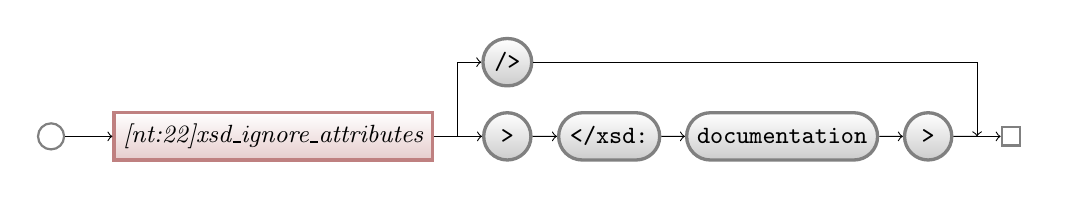
\begin{tikzpicture}
  \matrix[column sep=\ruleMatrixColumnSeparation, row sep=\ruleMatrixRowSeparation] {
    & & & & \node (p1-4) [terminal] {/>}; & \\
    \node (P0start) [firstPoint] {}; & & \node (p0-2) [nonterminal] {\nonTerminalSymbol{xsd\_ignore\_attributes}{22}}; & \node (p0-3) [point] {}; & \node (p0-4) [terminal] {>}; & \node (p0-5) [terminal] {</xsd:}; & \node (p0-6) [terminal] {documentation}; & \node (p0-7) [terminal] {>}; & \node (p0-8) [point] {}; & \node (p0-9) [lastPoint] {}; & \\
  };
  \draw[->] (P0start) -- (p0-2) ;
  \draw[->] (p0-2) -- (p0-4) ;
  \draw[->] (p0-4) -- (p0-5) ;
  \draw[->] (p0-5) -- (p0-6) ;
  \draw[->] (p0-6) -- (p0-7) ;
  \draw[->] (p0-3) |- (p1-4) ;
  \draw (p0-7) -- (p0-8) ;
  \draw[->] (p1-4) -| (p0-8) ;
  \draw[->] (p0-8) -- (p0-9) ;
\end{tikzpicture}

\nonTerminalSection{xsd\_element}{9}

\ruleSubsection{arxmlmetaparser\_syntax}{arxmlmetaparser\_syntax}{388}

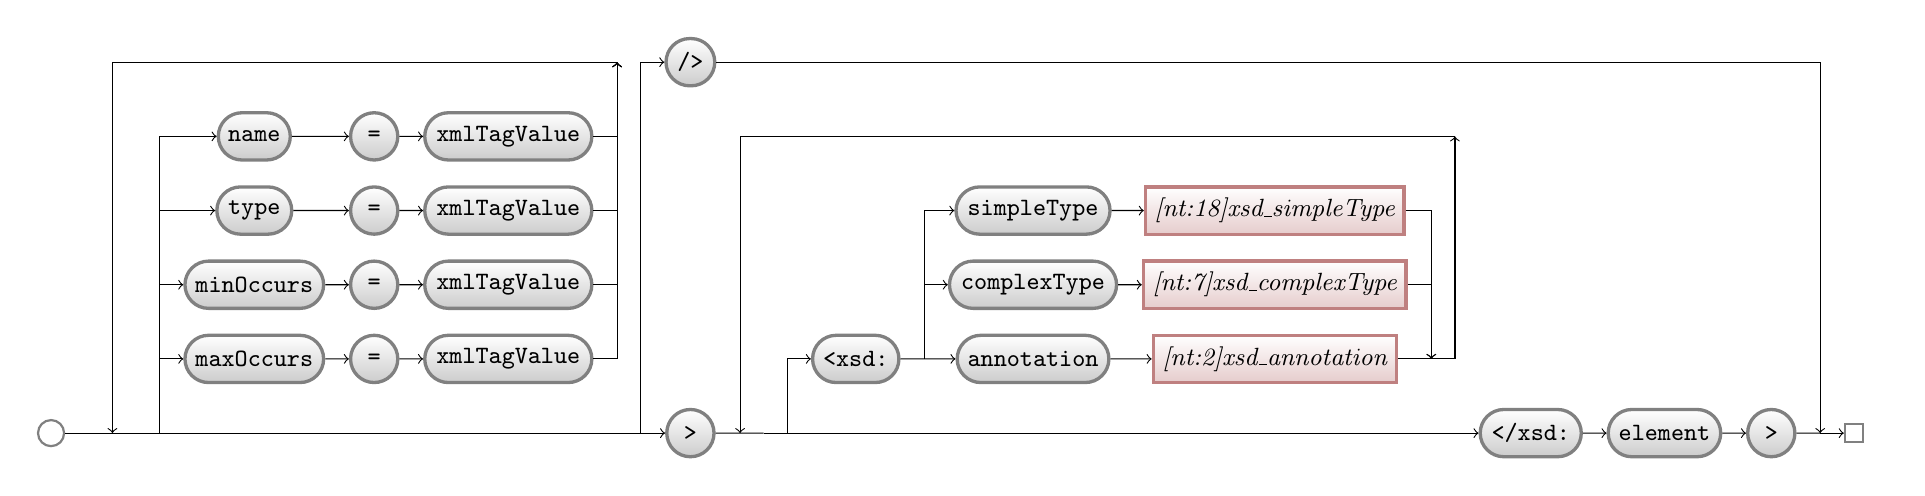
\begin{tikzpicture}
  \matrix[column sep=\ruleMatrixColumnSeparation, row sep=\ruleMatrixRowSeparation] {
    & & & & & & & & \node (p5-8) [point] {}; & & \node (p5-10) [terminal] {/>}; & \\
    & & & & & \node (p4-5) [terminal] {name}; & \node (p4-6) [terminal] {=}; & \node (p4-7) [terminal] {xmlTagValue}; & & & & & & & & & & & & \node (p4-19) [point] {}; & \\
    & & & & & \node (p3-5) [terminal] {type}; & \node (p3-6) [terminal] {=}; & \node (p3-7) [terminal] {xmlTagValue}; & & & & & & & & & \node (p3-16) [terminal] {simpleType}; & \node (p3-17) [nonterminal] {\nonTerminalSymbol{xsd\_simpleType}{18}}; & \\
    & & & & & \node (p2-5) [terminal] {minOccurs}; & \node (p2-6) [terminal] {=}; & \node (p2-7) [terminal] {xmlTagValue}; & & & & & & & & & \node (p2-16) [terminal] {complexType}; & \node (p2-17) [nonterminal] {\nonTerminalSymbol{xsd\_complexType}{7}}; & \\
    & & & & & \node (p1-5) [terminal] {maxOccurs}; & \node (p1-6) [terminal] {=}; & \node (p1-7) [terminal] {xmlTagValue}; & & & & & & & \node (p1-14) [terminal] {<xsd:}; & \node (p1-15) [point] {}; & \node (p1-16) [terminal] {annotation}; & \node (p1-17) [nonterminal] {\nonTerminalSymbol{xsd\_annotation}{2}}; & \node (p1-18) [point] {}; & \\
    \node (P0start) [firstPoint] {}; & & \node (p0-2) [point] {}; & \node (p0-3) [point] {}; & \node (p0-4) [point] {}; & & & & & \node (p0-9) [point] {}; & \node (p0-10) [terminal] {>}; & \node (p0-11) [point] {}; & \node (p0-12) [point] {}; & \node (p0-13) [point] {}; & & & & & & & \node (p0-20) [terminal] {</xsd:}; & \node (p0-21) [terminal] {element}; & \node (p0-22) [terminal] {>}; & \node (p0-23) [point] {}; & \node (p0-24) [lastPoint] {}; & \\
  };
  \draw (P0start) -- (p0-3) ;
  \draw[->] (p0-4) |- (p1-5) ;
  \draw[->] (p1-5) -- (p1-6) ;
  \draw[->] (p1-6) -- (p1-7) ;
  \draw[->] (p0-4) |- (p2-5) ;
  \draw[->] (p2-5) -- (p2-6) ;
  \draw[->] (p2-6) -- (p2-7) ;
  \draw[->] (p0-4) |- (p3-5) ;
  \draw[->] (p3-5) -- (p3-6) ;
  \draw[->] (p3-6) -- (p3-7) ;
  \draw[->] (p0-4) |- (p4-5) ;
  \draw[->] (p4-5) -- (p4-6) ;
  \draw[->] (p4-6) -- (p4-7) ;
  \draw[->] (p5-8) -| (p0-2) ;
  \draw[->] (p1-7) -| (p5-8) ;
  \draw[->] (p2-7) -| (p5-8) ;
  \draw[->] (p3-7) -| (p5-8) ;
  \draw[->] (p4-7) -| (p5-8) ;
  \draw[->] (p0-3) -- (p0-10) ;
  \draw (p0-10) -- (p0-12) ;
  \draw[->] (p0-13) |- (p1-14) ;
  \draw[->] (p1-14) -- (p1-16) ;
  \draw[->] (p1-16) -- (p1-17) ;
  \draw[->] (p1-15) |- (p2-16) ;
  \draw[->] (p2-16) -- (p2-17) ;
  \draw[->] (p1-15) |- (p3-16) ;
  \draw[->] (p3-16) -- (p3-17) ;
  \draw (p1-17) -- (p1-18) ;
  \draw[->] (p2-17) -| (p1-18) ;
  \draw[->] (p3-17) -| (p1-18) ;
  \draw[->] (p4-19) -| (p0-11) ;
  \draw[->] (p1-18) -| (p4-19) ;
  \draw[->] (p0-12) -- (p0-20) ;
  \draw[->] (p0-20) -- (p0-21) ;
  \draw[->] (p0-21) -- (p0-22) ;
  \draw[->] (p0-9) |- (p5-10) ;
  \draw (p0-22) -- (p0-23) ;
  \draw[->] (p5-10) -| (p0-23) ;
  \draw[->] (p0-23) -- (p0-24) ;
\end{tikzpicture}

\nonTerminalSection{xsd\_enumeration}{10}

\ruleSubsection{arxmlmetaparser\_syntax}{arxmlmetaparser\_syntax}{495}

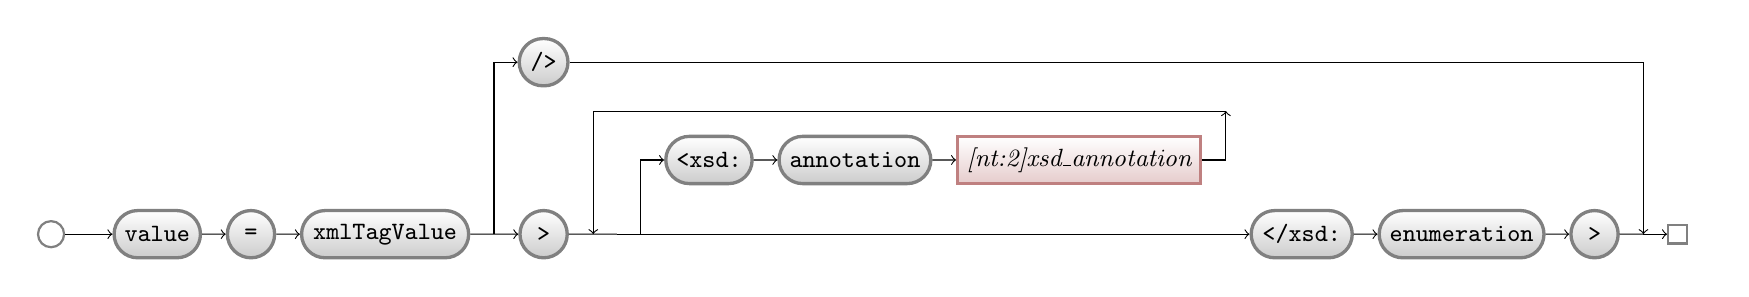
\begin{tikzpicture}
  \matrix[column sep=\ruleMatrixColumnSeparation, row sep=\ruleMatrixRowSeparation] {
    & & & & & & \node (p3-6) [terminal] {/>}; & \\
    & & & & & & & & & & & & & \node (p2-13) [point] {}; & \\
    & & & & & & & & & & \node (p1-10) [terminal] {<xsd:}; & \node (p1-11) [terminal] {annotation}; & \node (p1-12) [nonterminal] {\nonTerminalSymbol{xsd\_annotation}{2}}; & \\
    \node (P0start) [firstPoint] {}; & & \node (p0-2) [terminal] {value}; & \node (p0-3) [terminal] {=}; & \node (p0-4) [terminal] {xmlTagValue}; & \node (p0-5) [point] {}; & \node (p0-6) [terminal] {>}; & \node (p0-7) [point] {}; & \node (p0-8) [point] {}; & \node (p0-9) [point] {}; & & & & & \node (p0-14) [terminal] {</xsd:}; & \node (p0-15) [terminal] {enumeration}; & \node (p0-16) [terminal] {>}; & \node (p0-17) [point] {}; & \node (p0-18) [lastPoint] {}; & \\
  };
  \draw[->] (P0start) -- (p0-2) ;
  \draw[->] (p0-2) -- (p0-3) ;
  \draw[->] (p0-3) -- (p0-4) ;
  \draw[->] (p0-4) -- (p0-6) ;
  \draw (p0-6) -- (p0-8) ;
  \draw[->] (p0-9) |- (p1-10) ;
  \draw[->] (p1-10) -- (p1-11) ;
  \draw[->] (p1-11) -- (p1-12) ;
  \draw[->] (p2-13) -| (p0-7) ;
  \draw[->] (p1-12) -| (p2-13) ;
  \draw[->] (p0-8) -- (p0-14) ;
  \draw[->] (p0-14) -- (p0-15) ;
  \draw[->] (p0-15) -- (p0-16) ;
  \draw[->] (p0-5) |- (p3-6) ;
  \draw (p0-16) -- (p0-17) ;
  \draw[->] (p3-6) -| (p0-17) ;
  \draw[->] (p0-17) -- (p0-18) ;
\end{tikzpicture}

\nonTerminalSection{xsd\_extension}{11}

\ruleSubsection{arxmlmetaparser\_syntax}{arxmlmetaparser\_syntax}{523}

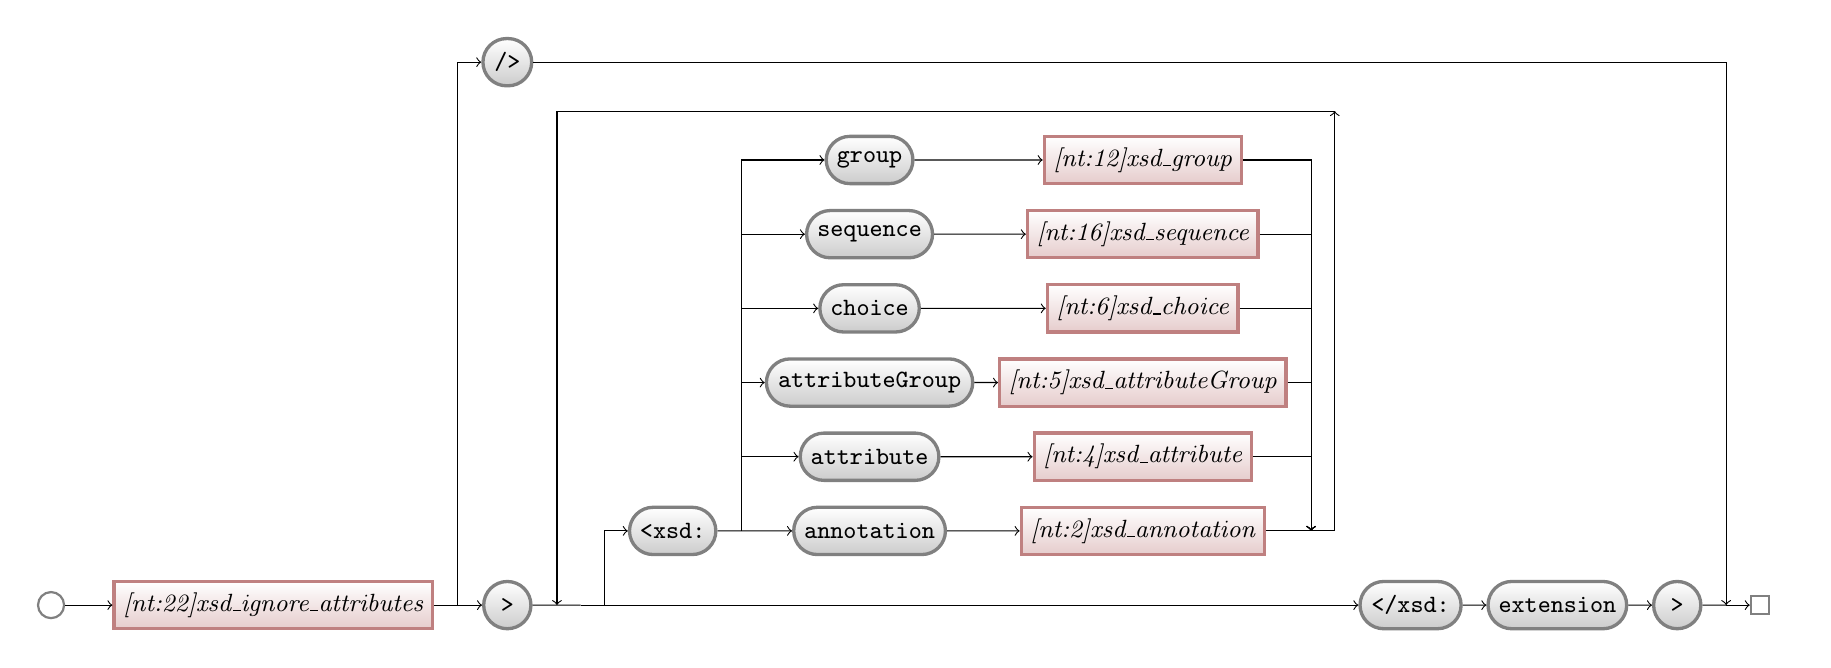
\begin{tikzpicture}
  \matrix[column sep=\ruleMatrixColumnSeparation, row sep=\ruleMatrixRowSeparation] {
    & & & & \node (p8-4) [terminal] {/>}; & \\
    & & & & & & & & & & & & & \node (p7-13) [point] {}; & \\
    & & & & & & & & & & \node (p6-10) [terminal] {group}; & \node (p6-11) [nonterminal] {\nonTerminalSymbol{xsd\_group}{12}}; & \\
    & & & & & & & & & & \node (p5-10) [terminal] {sequence}; & \node (p5-11) [nonterminal] {\nonTerminalSymbol{xsd\_sequence}{16}}; & \\
    & & & & & & & & & & \node (p4-10) [terminal] {choice}; & \node (p4-11) [nonterminal] {\nonTerminalSymbol{xsd\_choice}{6}}; & \\
    & & & & & & & & & & \node (p3-10) [terminal] {attributeGroup}; & \node (p3-11) [nonterminal] {\nonTerminalSymbol{xsd\_attributeGroup}{5}}; & \\
    & & & & & & & & & & \node (p2-10) [terminal] {attribute}; & \node (p2-11) [nonterminal] {\nonTerminalSymbol{xsd\_attribute}{4}}; & \\
    & & & & & & & & \node (p1-8) [terminal] {<xsd:}; & \node (p1-9) [point] {}; & \node (p1-10) [terminal] {annotation}; & \node (p1-11) [nonterminal] {\nonTerminalSymbol{xsd\_annotation}{2}}; & \node (p1-12) [point] {}; & \\
    \node (P0start) [firstPoint] {}; & & \node (p0-2) [nonterminal] {\nonTerminalSymbol{xsd\_ignore\_attributes}{22}}; & \node (p0-3) [point] {}; & \node (p0-4) [terminal] {>}; & \node (p0-5) [point] {}; & \node (p0-6) [point] {}; & \node (p0-7) [point] {}; & & & & & & & \node (p0-14) [terminal] {</xsd:}; & \node (p0-15) [terminal] {extension}; & \node (p0-16) [terminal] {>}; & \node (p0-17) [point] {}; & \node (p0-18) [lastPoint] {}; & \\
  };
  \draw[->] (P0start) -- (p0-2) ;
  \draw[->] (p0-2) -- (p0-4) ;
  \draw (p0-4) -- (p0-6) ;
  \draw[->] (p0-7) |- (p1-8) ;
  \draw[->] (p1-8) -- (p1-10) ;
  \draw[->] (p1-10) -- (p1-11) ;
  \draw[->] (p1-9) |- (p2-10) ;
  \draw[->] (p2-10) -- (p2-11) ;
  \draw[->] (p1-9) |- (p3-10) ;
  \draw[->] (p3-10) -- (p3-11) ;
  \draw[->] (p1-9) |- (p4-10) ;
  \draw[->] (p4-10) -- (p4-11) ;
  \draw[->] (p1-9) |- (p5-10) ;
  \draw[->] (p5-10) -- (p5-11) ;
  \draw[->] (p1-9) |- (p6-10) ;
  \draw[->] (p6-10) -- (p6-11) ;
  \draw (p1-11) -- (p1-12) ;
  \draw[->] (p2-11) -| (p1-12) ;
  \draw[->] (p3-11) -| (p1-12) ;
  \draw[->] (p4-11) -| (p1-12) ;
  \draw[->] (p5-11) -| (p1-12) ;
  \draw[->] (p6-11) -| (p1-12) ;
  \draw[->] (p7-13) -| (p0-5) ;
  \draw[->] (p1-12) -| (p7-13) ;
  \draw[->] (p0-6) -- (p0-14) ;
  \draw[->] (p0-14) -- (p0-15) ;
  \draw[->] (p0-15) -- (p0-16) ;
  \draw[->] (p0-3) |- (p8-4) ;
  \draw (p0-16) -- (p0-17) ;
  \draw[->] (p8-4) -| (p0-17) ;
  \draw[->] (p0-17) -- (p0-18) ;
\end{tikzpicture}

\nonTerminalSection{xsd\_group}{12}

\ruleSubsection{arxmlmetaparser\_syntax}{arxmlmetaparser\_syntax}{558}

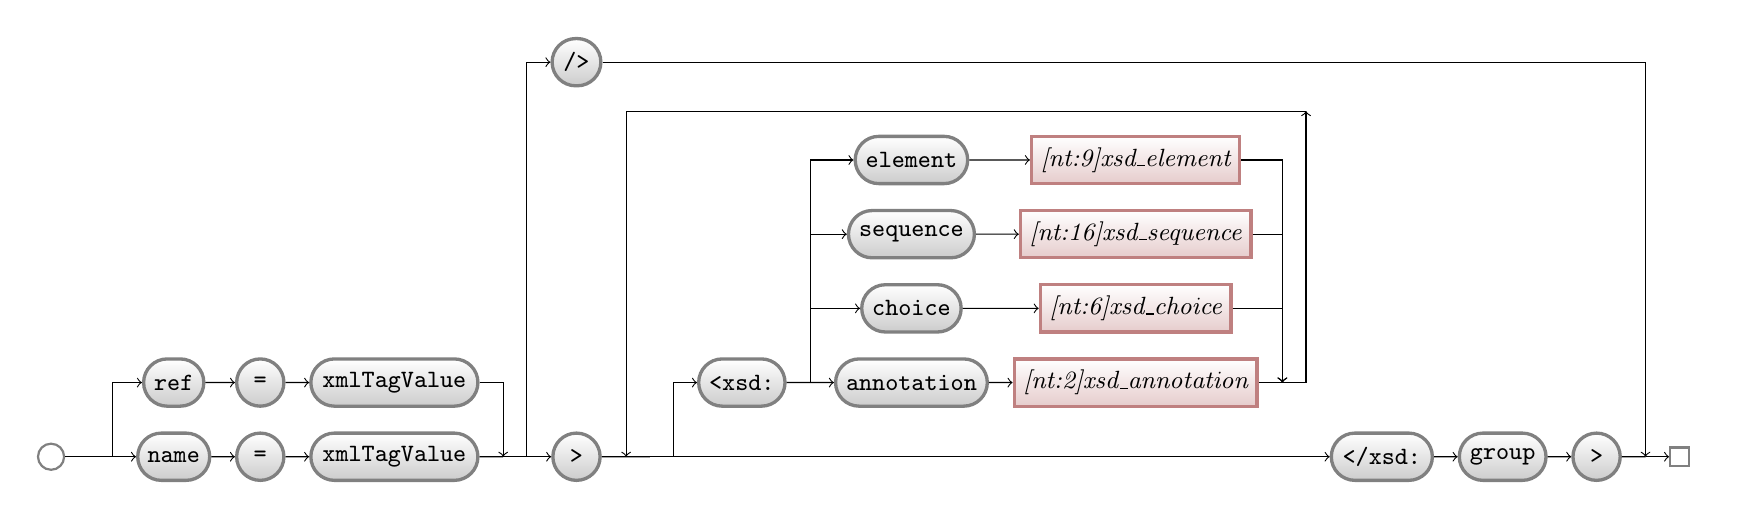
\begin{tikzpicture}
  \matrix[column sep=\ruleMatrixColumnSeparation, row sep=\ruleMatrixRowSeparation] {
    & & & & & & & & \node (p6-8) [terminal] {/>}; & \\
    & & & & & & & & & & & & & & & & & \node (p5-17) [point] {}; & \\
    & & & & & & & & & & & & & & \node (p4-14) [terminal] {element}; & \node (p4-15) [nonterminal] {\nonTerminalSymbol{xsd\_element}{9}}; & \\
    & & & & & & & & & & & & & & \node (p3-14) [terminal] {sequence}; & \node (p3-15) [nonterminal] {\nonTerminalSymbol{xsd\_sequence}{16}}; & \\
    & & & & & & & & & & & & & & \node (p2-14) [terminal] {choice}; & \node (p2-15) [nonterminal] {\nonTerminalSymbol{xsd\_choice}{6}}; & \\
    & & & \node (p1-3) [terminal] {ref}; & \node (p1-4) [terminal] {=}; & \node (p1-5) [terminal] {xmlTagValue}; & & & & & & & \node (p1-12) [terminal] {<xsd:}; & \node (p1-13) [point] {}; & \node (p1-14) [terminal] {annotation}; & \node (p1-15) [nonterminal] {\nonTerminalSymbol{xsd\_annotation}{2}}; & \node (p1-16) [point] {}; & \\
    \node (P0start) [firstPoint] {}; & & \node (p0-2) [point] {}; & \node (p0-3) [terminal] {name}; & \node (p0-4) [terminal] {=}; & \node (p0-5) [terminal] {xmlTagValue}; & \node (p0-6) [point] {}; & \node (p0-7) [point] {}; & \node (p0-8) [terminal] {>}; & \node (p0-9) [point] {}; & \node (p0-10) [point] {}; & \node (p0-11) [point] {}; & & & & & & & \node (p0-18) [terminal] {</xsd:}; & \node (p0-19) [terminal] {group}; & \node (p0-20) [terminal] {>}; & \node (p0-21) [point] {}; & \node (p0-22) [lastPoint] {}; & \\
  };
  \draw[->] (P0start) -- (p0-3) ;
  \draw[->] (p0-3) -- (p0-4) ;
  \draw[->] (p0-4) -- (p0-5) ;
  \draw[->] (p0-2) |- (p1-3) ;
  \draw[->] (p1-3) -- (p1-4) ;
  \draw[->] (p1-4) -- (p1-5) ;
  \draw (p0-5) -- (p0-6) ;
  \draw[->] (p1-5) -| (p0-6) ;
  \draw[->] (p0-6) -- (p0-8) ;
  \draw (p0-8) -- (p0-10) ;
  \draw[->] (p0-11) |- (p1-12) ;
  \draw[->] (p1-12) -- (p1-14) ;
  \draw[->] (p1-14) -- (p1-15) ;
  \draw[->] (p1-13) |- (p2-14) ;
  \draw[->] (p2-14) -- (p2-15) ;
  \draw[->] (p1-13) |- (p3-14) ;
  \draw[->] (p3-14) -- (p3-15) ;
  \draw[->] (p1-13) |- (p4-14) ;
  \draw[->] (p4-14) -- (p4-15) ;
  \draw (p1-15) -- (p1-16) ;
  \draw[->] (p2-15) -| (p1-16) ;
  \draw[->] (p3-15) -| (p1-16) ;
  \draw[->] (p4-15) -| (p1-16) ;
  \draw[->] (p5-17) -| (p0-9) ;
  \draw[->] (p1-16) -| (p5-17) ;
  \draw[->] (p0-10) -- (p0-18) ;
  \draw[->] (p0-18) -- (p0-19) ;
  \draw[->] (p0-19) -- (p0-20) ;
  \draw[->] (p0-7) |- (p6-8) ;
  \draw (p0-20) -- (p0-21) ;
  \draw[->] (p6-8) -| (p0-21) ;
  \draw[->] (p0-21) -- (p0-22) ;
\end{tikzpicture}

\nonTerminalSection{xsd\_ignore\_attributes}{22}

\ruleSubsection{arxmlmetaparser\_syntax}{arxmlmetaparser\_syntax}{1011}

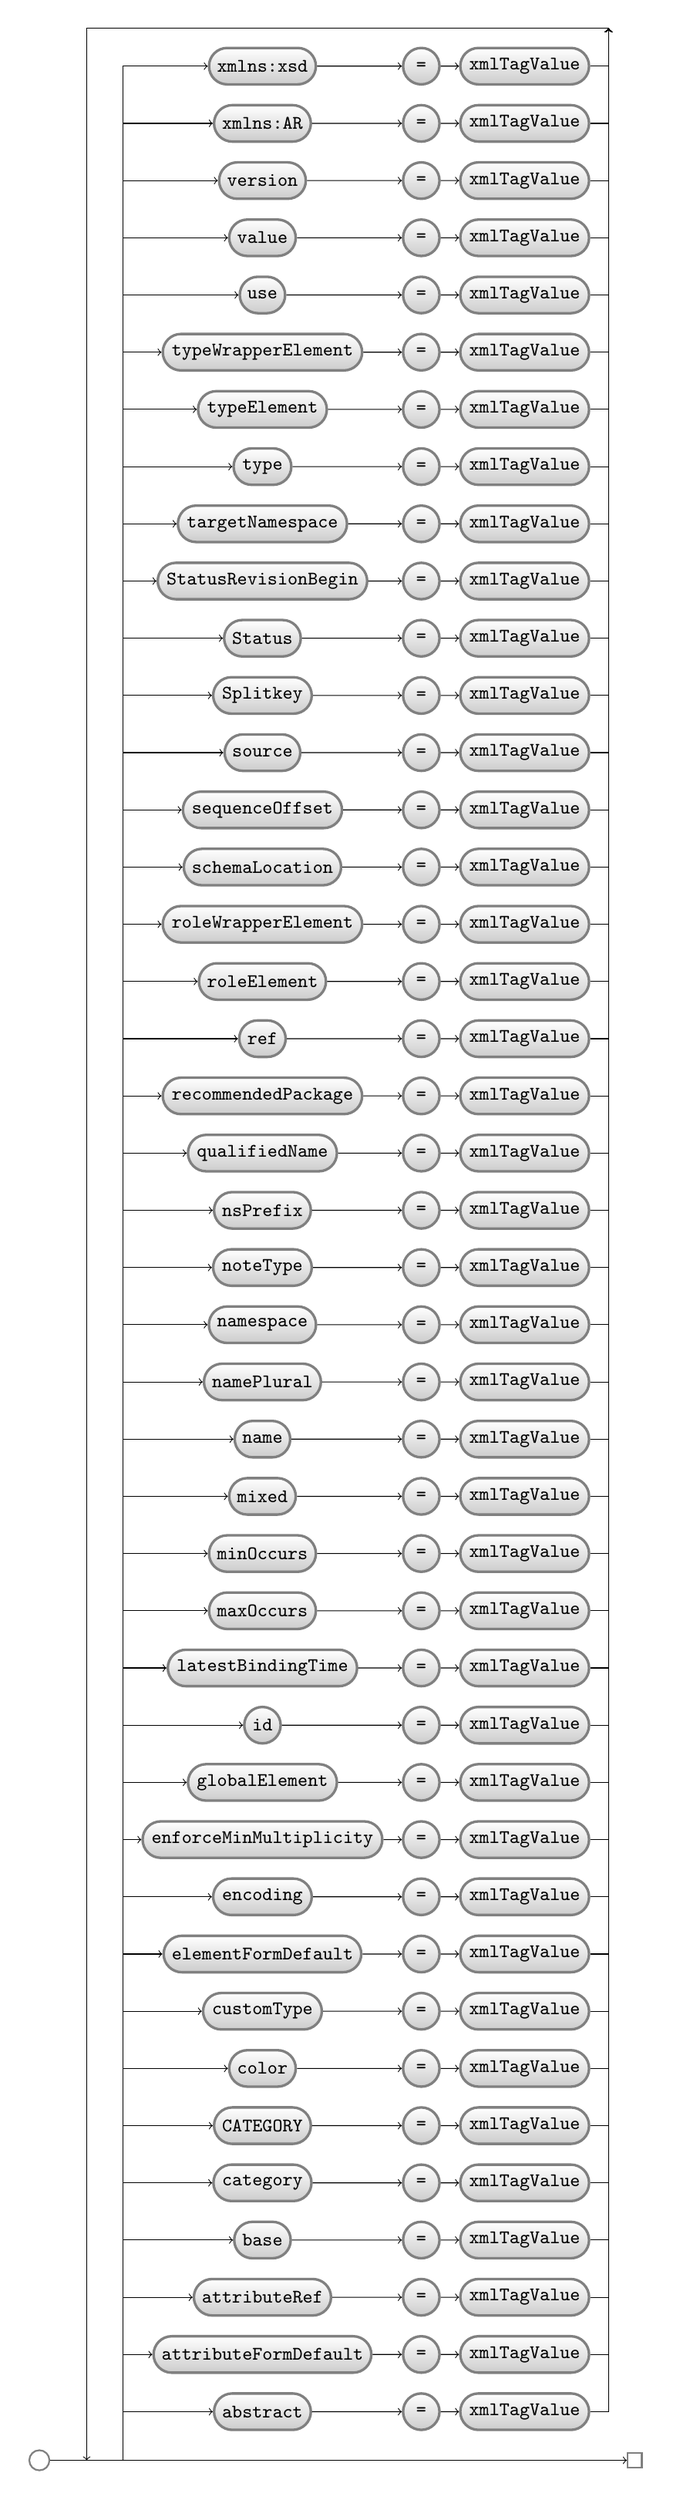
\begin{tikzpicture}
  \matrix[column sep=\ruleMatrixColumnSeparation, row sep=\ruleMatrixRowSeparation] {
    & & & & & & & & \node (p43-8) [point] {}; & \\
    & & & & & \node (p42-5) [terminal] {xmlns:xsd}; & \node (p42-6) [terminal] {=}; & \node (p42-7) [terminal] {xmlTagValue}; & \\
    & & & & & \node (p41-5) [terminal] {xmlns:AR}; & \node (p41-6) [terminal] {=}; & \node (p41-7) [terminal] {xmlTagValue}; & \\
    & & & & & \node (p40-5) [terminal] {version}; & \node (p40-6) [terminal] {=}; & \node (p40-7) [terminal] {xmlTagValue}; & \\
    & & & & & \node (p39-5) [terminal] {value}; & \node (p39-6) [terminal] {=}; & \node (p39-7) [terminal] {xmlTagValue}; & \\
    & & & & & \node (p38-5) [terminal] {use}; & \node (p38-6) [terminal] {=}; & \node (p38-7) [terminal] {xmlTagValue}; & \\
    & & & & & \node (p37-5) [terminal] {typeWrapperElement}; & \node (p37-6) [terminal] {=}; & \node (p37-7) [terminal] {xmlTagValue}; & \\
    & & & & & \node (p36-5) [terminal] {typeElement}; & \node (p36-6) [terminal] {=}; & \node (p36-7) [terminal] {xmlTagValue}; & \\
    & & & & & \node (p35-5) [terminal] {type}; & \node (p35-6) [terminal] {=}; & \node (p35-7) [terminal] {xmlTagValue}; & \\
    & & & & & \node (p34-5) [terminal] {targetNamespace}; & \node (p34-6) [terminal] {=}; & \node (p34-7) [terminal] {xmlTagValue}; & \\
    & & & & & \node (p33-5) [terminal] {StatusRevisionBegin}; & \node (p33-6) [terminal] {=}; & \node (p33-7) [terminal] {xmlTagValue}; & \\
    & & & & & \node (p32-5) [terminal] {Status}; & \node (p32-6) [terminal] {=}; & \node (p32-7) [terminal] {xmlTagValue}; & \\
    & & & & & \node (p31-5) [terminal] {Splitkey}; & \node (p31-6) [terminal] {=}; & \node (p31-7) [terminal] {xmlTagValue}; & \\
    & & & & & \node (p30-5) [terminal] {source}; & \node (p30-6) [terminal] {=}; & \node (p30-7) [terminal] {xmlTagValue}; & \\
    & & & & & \node (p29-5) [terminal] {sequenceOffset}; & \node (p29-6) [terminal] {=}; & \node (p29-7) [terminal] {xmlTagValue}; & \\
    & & & & & \node (p28-5) [terminal] {schemaLocation}; & \node (p28-6) [terminal] {=}; & \node (p28-7) [terminal] {xmlTagValue}; & \\
    & & & & & \node (p27-5) [terminal] {roleWrapperElement}; & \node (p27-6) [terminal] {=}; & \node (p27-7) [terminal] {xmlTagValue}; & \\
    & & & & & \node (p26-5) [terminal] {roleElement}; & \node (p26-6) [terminal] {=}; & \node (p26-7) [terminal] {xmlTagValue}; & \\
    & & & & & \node (p25-5) [terminal] {ref}; & \node (p25-6) [terminal] {=}; & \node (p25-7) [terminal] {xmlTagValue}; & \\
    & & & & & \node (p24-5) [terminal] {recommendedPackage}; & \node (p24-6) [terminal] {=}; & \node (p24-7) [terminal] {xmlTagValue}; & \\
    & & & & & \node (p23-5) [terminal] {qualifiedName}; & \node (p23-6) [terminal] {=}; & \node (p23-7) [terminal] {xmlTagValue}; & \\
    & & & & & \node (p22-5) [terminal] {nsPrefix}; & \node (p22-6) [terminal] {=}; & \node (p22-7) [terminal] {xmlTagValue}; & \\
    & & & & & \node (p21-5) [terminal] {noteType}; & \node (p21-6) [terminal] {=}; & \node (p21-7) [terminal] {xmlTagValue}; & \\
    & & & & & \node (p20-5) [terminal] {namespace}; & \node (p20-6) [terminal] {=}; & \node (p20-7) [terminal] {xmlTagValue}; & \\
    & & & & & \node (p19-5) [terminal] {namePlural}; & \node (p19-6) [terminal] {=}; & \node (p19-7) [terminal] {xmlTagValue}; & \\
    & & & & & \node (p18-5) [terminal] {name}; & \node (p18-6) [terminal] {=}; & \node (p18-7) [terminal] {xmlTagValue}; & \\
    & & & & & \node (p17-5) [terminal] {mixed}; & \node (p17-6) [terminal] {=}; & \node (p17-7) [terminal] {xmlTagValue}; & \\
    & & & & & \node (p16-5) [terminal] {minOccurs}; & \node (p16-6) [terminal] {=}; & \node (p16-7) [terminal] {xmlTagValue}; & \\
    & & & & & \node (p15-5) [terminal] {maxOccurs}; & \node (p15-6) [terminal] {=}; & \node (p15-7) [terminal] {xmlTagValue}; & \\
    & & & & & \node (p14-5) [terminal] {latestBindingTime}; & \node (p14-6) [terminal] {=}; & \node (p14-7) [terminal] {xmlTagValue}; & \\
    & & & & & \node (p13-5) [terminal] {id}; & \node (p13-6) [terminal] {=}; & \node (p13-7) [terminal] {xmlTagValue}; & \\
    & & & & & \node (p12-5) [terminal] {globalElement}; & \node (p12-6) [terminal] {=}; & \node (p12-7) [terminal] {xmlTagValue}; & \\
    & & & & & \node (p11-5) [terminal] {enforceMinMultiplicity}; & \node (p11-6) [terminal] {=}; & \node (p11-7) [terminal] {xmlTagValue}; & \\
    & & & & & \node (p10-5) [terminal] {encoding}; & \node (p10-6) [terminal] {=}; & \node (p10-7) [terminal] {xmlTagValue}; & \\
    & & & & & \node (p9-5) [terminal] {elementFormDefault}; & \node (p9-6) [terminal] {=}; & \node (p9-7) [terminal] {xmlTagValue}; & \\
    & & & & & \node (p8-5) [terminal] {customType}; & \node (p8-6) [terminal] {=}; & \node (p8-7) [terminal] {xmlTagValue}; & \\
    & & & & & \node (p7-5) [terminal] {color}; & \node (p7-6) [terminal] {=}; & \node (p7-7) [terminal] {xmlTagValue}; & \\
    & & & & & \node (p6-5) [terminal] {CATEGORY}; & \node (p6-6) [terminal] {=}; & \node (p6-7) [terminal] {xmlTagValue}; & \\
    & & & & & \node (p5-5) [terminal] {category}; & \node (p5-6) [terminal] {=}; & \node (p5-7) [terminal] {xmlTagValue}; & \\
    & & & & & \node (p4-5) [terminal] {base}; & \node (p4-6) [terminal] {=}; & \node (p4-7) [terminal] {xmlTagValue}; & \\
    & & & & & \node (p3-5) [terminal] {attributeRef}; & \node (p3-6) [terminal] {=}; & \node (p3-7) [terminal] {xmlTagValue}; & \\
    & & & & & \node (p2-5) [terminal] {attributeFormDefault}; & \node (p2-6) [terminal] {=}; & \node (p2-7) [terminal] {xmlTagValue}; & \\
    & & & & & \node (p1-5) [terminal] {abstract}; & \node (p1-6) [terminal] {=}; & \node (p1-7) [terminal] {xmlTagValue}; & \\
    \node (P0start) [firstPoint] {}; & & \node (p0-2) [point] {}; & \node (p0-3) [point] {}; & \node (p0-4) [point] {}; & & & & & \node (p0-9) [lastPoint] {}; & \\
  };
  \draw (P0start) -- (p0-3) ;
  \draw[->] (p0-4) |- (p1-5) ;
  \draw[->] (p1-5) -- (p1-6) ;
  \draw[->] (p1-6) -- (p1-7) ;
  \draw[->] (p0-4) |- (p2-5) ;
  \draw[->] (p2-5) -- (p2-6) ;
  \draw[->] (p2-6) -- (p2-7) ;
  \draw[->] (p0-4) |- (p3-5) ;
  \draw[->] (p3-5) -- (p3-6) ;
  \draw[->] (p3-6) -- (p3-7) ;
  \draw[->] (p0-4) |- (p4-5) ;
  \draw[->] (p4-5) -- (p4-6) ;
  \draw[->] (p4-6) -- (p4-7) ;
  \draw[->] (p0-4) |- (p5-5) ;
  \draw[->] (p5-5) -- (p5-6) ;
  \draw[->] (p5-6) -- (p5-7) ;
  \draw[->] (p0-4) |- (p6-5) ;
  \draw[->] (p6-5) -- (p6-6) ;
  \draw[->] (p6-6) -- (p6-7) ;
  \draw[->] (p0-4) |- (p7-5) ;
  \draw[->] (p7-5) -- (p7-6) ;
  \draw[->] (p7-6) -- (p7-7) ;
  \draw[->] (p0-4) |- (p8-5) ;
  \draw[->] (p8-5) -- (p8-6) ;
  \draw[->] (p8-6) -- (p8-7) ;
  \draw[->] (p0-4) |- (p9-5) ;
  \draw[->] (p9-5) -- (p9-6) ;
  \draw[->] (p9-6) -- (p9-7) ;
  \draw[->] (p0-4) |- (p10-5) ;
  \draw[->] (p10-5) -- (p10-6) ;
  \draw[->] (p10-6) -- (p10-7) ;
  \draw[->] (p0-4) |- (p11-5) ;
  \draw[->] (p11-5) -- (p11-6) ;
  \draw[->] (p11-6) -- (p11-7) ;
  \draw[->] (p0-4) |- (p12-5) ;
  \draw[->] (p12-5) -- (p12-6) ;
  \draw[->] (p12-6) -- (p12-7) ;
  \draw[->] (p0-4) |- (p13-5) ;
  \draw[->] (p13-5) -- (p13-6) ;
  \draw[->] (p13-6) -- (p13-7) ;
  \draw[->] (p0-4) |- (p14-5) ;
  \draw[->] (p14-5) -- (p14-6) ;
  \draw[->] (p14-6) -- (p14-7) ;
  \draw[->] (p0-4) |- (p15-5) ;
  \draw[->] (p15-5) -- (p15-6) ;
  \draw[->] (p15-6) -- (p15-7) ;
  \draw[->] (p0-4) |- (p16-5) ;
  \draw[->] (p16-5) -- (p16-6) ;
  \draw[->] (p16-6) -- (p16-7) ;
  \draw[->] (p0-4) |- (p17-5) ;
  \draw[->] (p17-5) -- (p17-6) ;
  \draw[->] (p17-6) -- (p17-7) ;
  \draw[->] (p0-4) |- (p18-5) ;
  \draw[->] (p18-5) -- (p18-6) ;
  \draw[->] (p18-6) -- (p18-7) ;
  \draw[->] (p0-4) |- (p19-5) ;
  \draw[->] (p19-5) -- (p19-6) ;
  \draw[->] (p19-6) -- (p19-7) ;
  \draw[->] (p0-4) |- (p20-5) ;
  \draw[->] (p20-5) -- (p20-6) ;
  \draw[->] (p20-6) -- (p20-7) ;
  \draw[->] (p0-4) |- (p21-5) ;
  \draw[->] (p21-5) -- (p21-6) ;
  \draw[->] (p21-6) -- (p21-7) ;
  \draw[->] (p0-4) |- (p22-5) ;
  \draw[->] (p22-5) -- (p22-6) ;
  \draw[->] (p22-6) -- (p22-7) ;
  \draw[->] (p0-4) |- (p23-5) ;
  \draw[->] (p23-5) -- (p23-6) ;
  \draw[->] (p23-6) -- (p23-7) ;
  \draw[->] (p0-4) |- (p24-5) ;
  \draw[->] (p24-5) -- (p24-6) ;
  \draw[->] (p24-6) -- (p24-7) ;
  \draw[->] (p0-4) |- (p25-5) ;
  \draw[->] (p25-5) -- (p25-6) ;
  \draw[->] (p25-6) -- (p25-7) ;
  \draw[->] (p0-4) |- (p26-5) ;
  \draw[->] (p26-5) -- (p26-6) ;
  \draw[->] (p26-6) -- (p26-7) ;
  \draw[->] (p0-4) |- (p27-5) ;
  \draw[->] (p27-5) -- (p27-6) ;
  \draw[->] (p27-6) -- (p27-7) ;
  \draw[->] (p0-4) |- (p28-5) ;
  \draw[->] (p28-5) -- (p28-6) ;
  \draw[->] (p28-6) -- (p28-7) ;
  \draw[->] (p0-4) |- (p29-5) ;
  \draw[->] (p29-5) -- (p29-6) ;
  \draw[->] (p29-6) -- (p29-7) ;
  \draw[->] (p0-4) |- (p30-5) ;
  \draw[->] (p30-5) -- (p30-6) ;
  \draw[->] (p30-6) -- (p30-7) ;
  \draw[->] (p0-4) |- (p31-5) ;
  \draw[->] (p31-5) -- (p31-6) ;
  \draw[->] (p31-6) -- (p31-7) ;
  \draw[->] (p0-4) |- (p32-5) ;
  \draw[->] (p32-5) -- (p32-6) ;
  \draw[->] (p32-6) -- (p32-7) ;
  \draw[->] (p0-4) |- (p33-5) ;
  \draw[->] (p33-5) -- (p33-6) ;
  \draw[->] (p33-6) -- (p33-7) ;
  \draw[->] (p0-4) |- (p34-5) ;
  \draw[->] (p34-5) -- (p34-6) ;
  \draw[->] (p34-6) -- (p34-7) ;
  \draw[->] (p0-4) |- (p35-5) ;
  \draw[->] (p35-5) -- (p35-6) ;
  \draw[->] (p35-6) -- (p35-7) ;
  \draw[->] (p0-4) |- (p36-5) ;
  \draw[->] (p36-5) -- (p36-6) ;
  \draw[->] (p36-6) -- (p36-7) ;
  \draw[->] (p0-4) |- (p37-5) ;
  \draw[->] (p37-5) -- (p37-6) ;
  \draw[->] (p37-6) -- (p37-7) ;
  \draw[->] (p0-4) |- (p38-5) ;
  \draw[->] (p38-5) -- (p38-6) ;
  \draw[->] (p38-6) -- (p38-7) ;
  \draw[->] (p0-4) |- (p39-5) ;
  \draw[->] (p39-5) -- (p39-6) ;
  \draw[->] (p39-6) -- (p39-7) ;
  \draw[->] (p0-4) |- (p40-5) ;
  \draw[->] (p40-5) -- (p40-6) ;
  \draw[->] (p40-6) -- (p40-7) ;
  \draw[->] (p0-4) |- (p41-5) ;
  \draw[->] (p41-5) -- (p41-6) ;
  \draw[->] (p41-6) -- (p41-7) ;
  \draw[->] (p0-4) |- (p42-5) ;
  \draw[->] (p42-5) -- (p42-6) ;
  \draw[->] (p42-6) -- (p42-7) ;
  \draw[->] (p43-8) -| (p0-2) ;
  \draw[->] (p1-7) -| (p43-8) ;
  \draw[->] (p2-7) -| (p43-8) ;
  \draw[->] (p3-7) -| (p43-8) ;
  \draw[->] (p4-7) -| (p43-8) ;
  \draw[->] (p5-7) -| (p43-8) ;
  \draw[->] (p6-7) -| (p43-8) ;
  \draw[->] (p7-7) -| (p43-8) ;
  \draw[->] (p8-7) -| (p43-8) ;
  \draw[->] (p9-7) -| (p43-8) ;
  \draw[->] (p10-7) -| (p43-8) ;
  \draw[->] (p11-7) -| (p43-8) ;
  \draw[->] (p12-7) -| (p43-8) ;
  \draw[->] (p13-7) -| (p43-8) ;
  \draw[->] (p14-7) -| (p43-8) ;
  \draw[->] (p15-7) -| (p43-8) ;
  \draw[->] (p16-7) -| (p43-8) ;
  \draw[->] (p17-7) -| (p43-8) ;
  \draw[->] (p18-7) -| (p43-8) ;
  \draw[->] (p19-7) -| (p43-8) ;
  \draw[->] (p20-7) -| (p43-8) ;
  \draw[->] (p21-7) -| (p43-8) ;
  \draw[->] (p22-7) -| (p43-8) ;
  \draw[->] (p23-7) -| (p43-8) ;
  \draw[->] (p24-7) -| (p43-8) ;
  \draw[->] (p25-7) -| (p43-8) ;
  \draw[->] (p26-7) -| (p43-8) ;
  \draw[->] (p27-7) -| (p43-8) ;
  \draw[->] (p28-7) -| (p43-8) ;
  \draw[->] (p29-7) -| (p43-8) ;
  \draw[->] (p30-7) -| (p43-8) ;
  \draw[->] (p31-7) -| (p43-8) ;
  \draw[->] (p32-7) -| (p43-8) ;
  \draw[->] (p33-7) -| (p43-8) ;
  \draw[->] (p34-7) -| (p43-8) ;
  \draw[->] (p35-7) -| (p43-8) ;
  \draw[->] (p36-7) -| (p43-8) ;
  \draw[->] (p37-7) -| (p43-8) ;
  \draw[->] (p38-7) -| (p43-8) ;
  \draw[->] (p39-7) -| (p43-8) ;
  \draw[->] (p40-7) -| (p43-8) ;
  \draw[->] (p41-7) -| (p43-8) ;
  \draw[->] (p42-7) -| (p43-8) ;
  \draw[->] (p0-3) -- (p0-9) ;
\end{tikzpicture}

\nonTerminalSection{xsd\_import}{13}

\ruleSubsection{arxmlmetaparser\_syntax}{arxmlmetaparser\_syntax}{630}

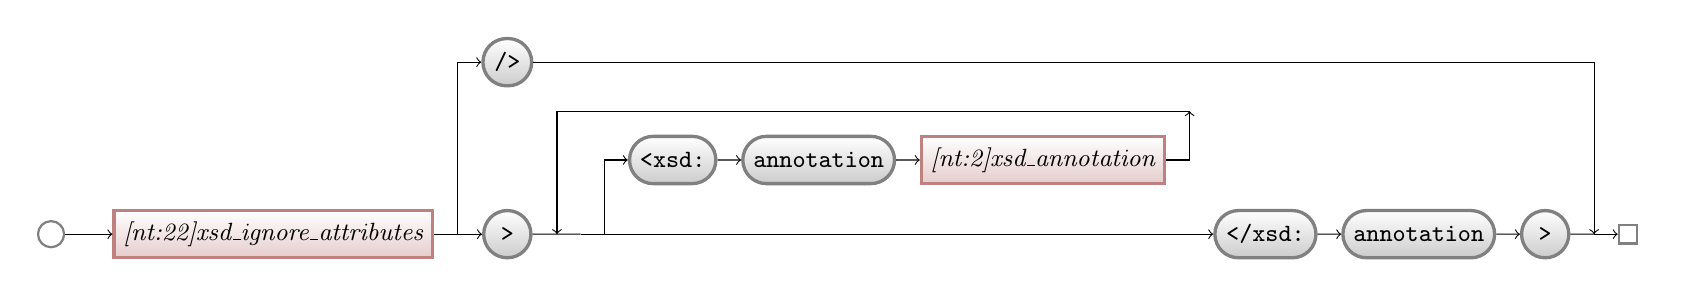
\begin{tikzpicture}
  \matrix[column sep=\ruleMatrixColumnSeparation, row sep=\ruleMatrixRowSeparation] {
    & & & & \node (p3-4) [terminal] {/>}; & \\
    & & & & & & & & & & & \node (p2-11) [point] {}; & \\
    & & & & & & & & \node (p1-8) [terminal] {<xsd:}; & \node (p1-9) [terminal] {annotation}; & \node (p1-10) [nonterminal] {\nonTerminalSymbol{xsd\_annotation}{2}}; & \\
    \node (P0start) [firstPoint] {}; & & \node (p0-2) [nonterminal] {\nonTerminalSymbol{xsd\_ignore\_attributes}{22}}; & \node (p0-3) [point] {}; & \node (p0-4) [terminal] {>}; & \node (p0-5) [point] {}; & \node (p0-6) [point] {}; & \node (p0-7) [point] {}; & & & & & \node (p0-12) [terminal] {</xsd:}; & \node (p0-13) [terminal] {annotation}; & \node (p0-14) [terminal] {>}; & \node (p0-15) [point] {}; & \node (p0-16) [lastPoint] {}; & \\
  };
  \draw[->] (P0start) -- (p0-2) ;
  \draw[->] (p0-2) -- (p0-4) ;
  \draw (p0-4) -- (p0-6) ;
  \draw[->] (p0-7) |- (p1-8) ;
  \draw[->] (p1-8) -- (p1-9) ;
  \draw[->] (p1-9) -- (p1-10) ;
  \draw[->] (p2-11) -| (p0-5) ;
  \draw[->] (p1-10) -| (p2-11) ;
  \draw[->] (p0-6) -- (p0-12) ;
  \draw[->] (p0-12) -- (p0-13) ;
  \draw[->] (p0-13) -- (p0-14) ;
  \draw[->] (p0-3) |- (p3-4) ;
  \draw (p0-14) -- (p0-15) ;
  \draw[->] (p3-4) -| (p0-15) ;
  \draw[->] (p0-15) -- (p0-16) ;
\end{tikzpicture}

\nonTerminalSection{xsd\_maxLength}{19}

\ruleSubsection{arxmlmetaparser\_syntax}{arxmlmetaparser\_syntax}{942}

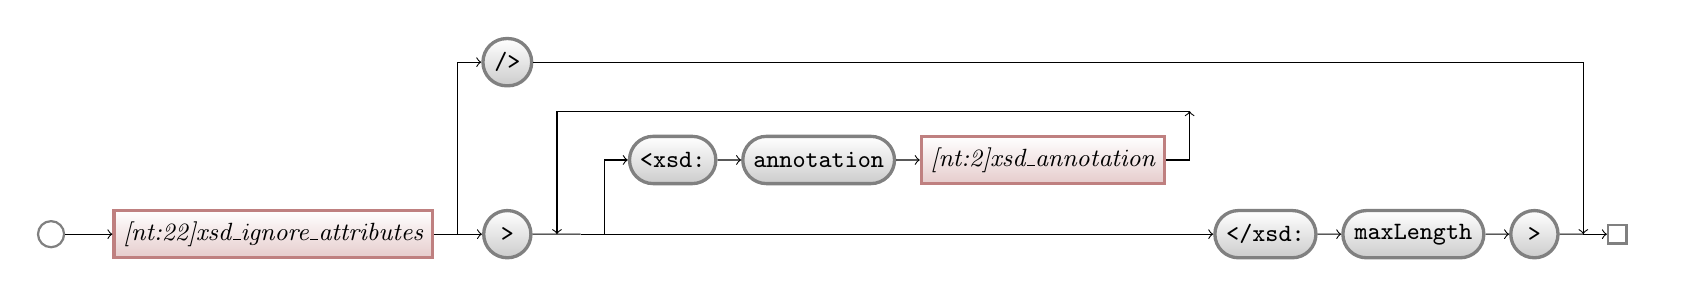
\begin{tikzpicture}
  \matrix[column sep=\ruleMatrixColumnSeparation, row sep=\ruleMatrixRowSeparation] {
    & & & & \node (p3-4) [terminal] {/>}; & \\
    & & & & & & & & & & & \node (p2-11) [point] {}; & \\
    & & & & & & & & \node (p1-8) [terminal] {<xsd:}; & \node (p1-9) [terminal] {annotation}; & \node (p1-10) [nonterminal] {\nonTerminalSymbol{xsd\_annotation}{2}}; & \\
    \node (P0start) [firstPoint] {}; & & \node (p0-2) [nonterminal] {\nonTerminalSymbol{xsd\_ignore\_attributes}{22}}; & \node (p0-3) [point] {}; & \node (p0-4) [terminal] {>}; & \node (p0-5) [point] {}; & \node (p0-6) [point] {}; & \node (p0-7) [point] {}; & & & & & \node (p0-12) [terminal] {</xsd:}; & \node (p0-13) [terminal] {maxLength}; & \node (p0-14) [terminal] {>}; & \node (p0-15) [point] {}; & \node (p0-16) [lastPoint] {}; & \\
  };
  \draw[->] (P0start) -- (p0-2) ;
  \draw[->] (p0-2) -- (p0-4) ;
  \draw (p0-4) -- (p0-6) ;
  \draw[->] (p0-7) |- (p1-8) ;
  \draw[->] (p1-8) -- (p1-9) ;
  \draw[->] (p1-9) -- (p1-10) ;
  \draw[->] (p2-11) -| (p0-5) ;
  \draw[->] (p1-10) -| (p2-11) ;
  \draw[->] (p0-6) -- (p0-12) ;
  \draw[->] (p0-12) -- (p0-13) ;
  \draw[->] (p0-13) -- (p0-14) ;
  \draw[->] (p0-3) |- (p3-4) ;
  \draw (p0-14) -- (p0-15) ;
  \draw[->] (p3-4) -| (p0-15) ;
  \draw[->] (p0-15) -- (p0-16) ;
\end{tikzpicture}

\nonTerminalSection{xsd\_pattern}{20}

\ruleSubsection{arxmlmetaparser\_syntax}{arxmlmetaparser\_syntax}{967}

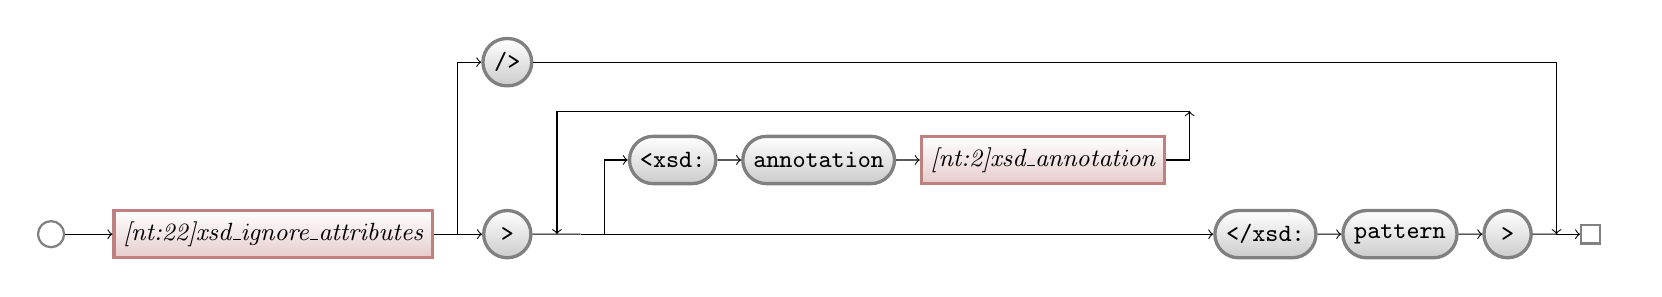
\begin{tikzpicture}
  \matrix[column sep=\ruleMatrixColumnSeparation, row sep=\ruleMatrixRowSeparation] {
    & & & & \node (p3-4) [terminal] {/>}; & \\
    & & & & & & & & & & & \node (p2-11) [point] {}; & \\
    & & & & & & & & \node (p1-8) [terminal] {<xsd:}; & \node (p1-9) [terminal] {annotation}; & \node (p1-10) [nonterminal] {\nonTerminalSymbol{xsd\_annotation}{2}}; & \\
    \node (P0start) [firstPoint] {}; & & \node (p0-2) [nonterminal] {\nonTerminalSymbol{xsd\_ignore\_attributes}{22}}; & \node (p0-3) [point] {}; & \node (p0-4) [terminal] {>}; & \node (p0-5) [point] {}; & \node (p0-6) [point] {}; & \node (p0-7) [point] {}; & & & & & \node (p0-12) [terminal] {</xsd:}; & \node (p0-13) [terminal] {pattern}; & \node (p0-14) [terminal] {>}; & \node (p0-15) [point] {}; & \node (p0-16) [lastPoint] {}; & \\
  };
  \draw[->] (P0start) -- (p0-2) ;
  \draw[->] (p0-2) -- (p0-4) ;
  \draw (p0-4) -- (p0-6) ;
  \draw[->] (p0-7) |- (p1-8) ;
  \draw[->] (p1-8) -- (p1-9) ;
  \draw[->] (p1-9) -- (p1-10) ;
  \draw[->] (p2-11) -| (p0-5) ;
  \draw[->] (p1-10) -| (p2-11) ;
  \draw[->] (p0-6) -- (p0-12) ;
  \draw[->] (p0-12) -- (p0-13) ;
  \draw[->] (p0-13) -- (p0-14) ;
  \draw[->] (p0-3) |- (p3-4) ;
  \draw (p0-14) -- (p0-15) ;
  \draw[->] (p3-4) -| (p0-15) ;
  \draw[->] (p0-15) -- (p0-16) ;
\end{tikzpicture}

\nonTerminalSection{xsd\_restriction}{14}

\ruleSubsection{arxmlmetaparser\_syntax}{arxmlmetaparser\_syntax}{653}

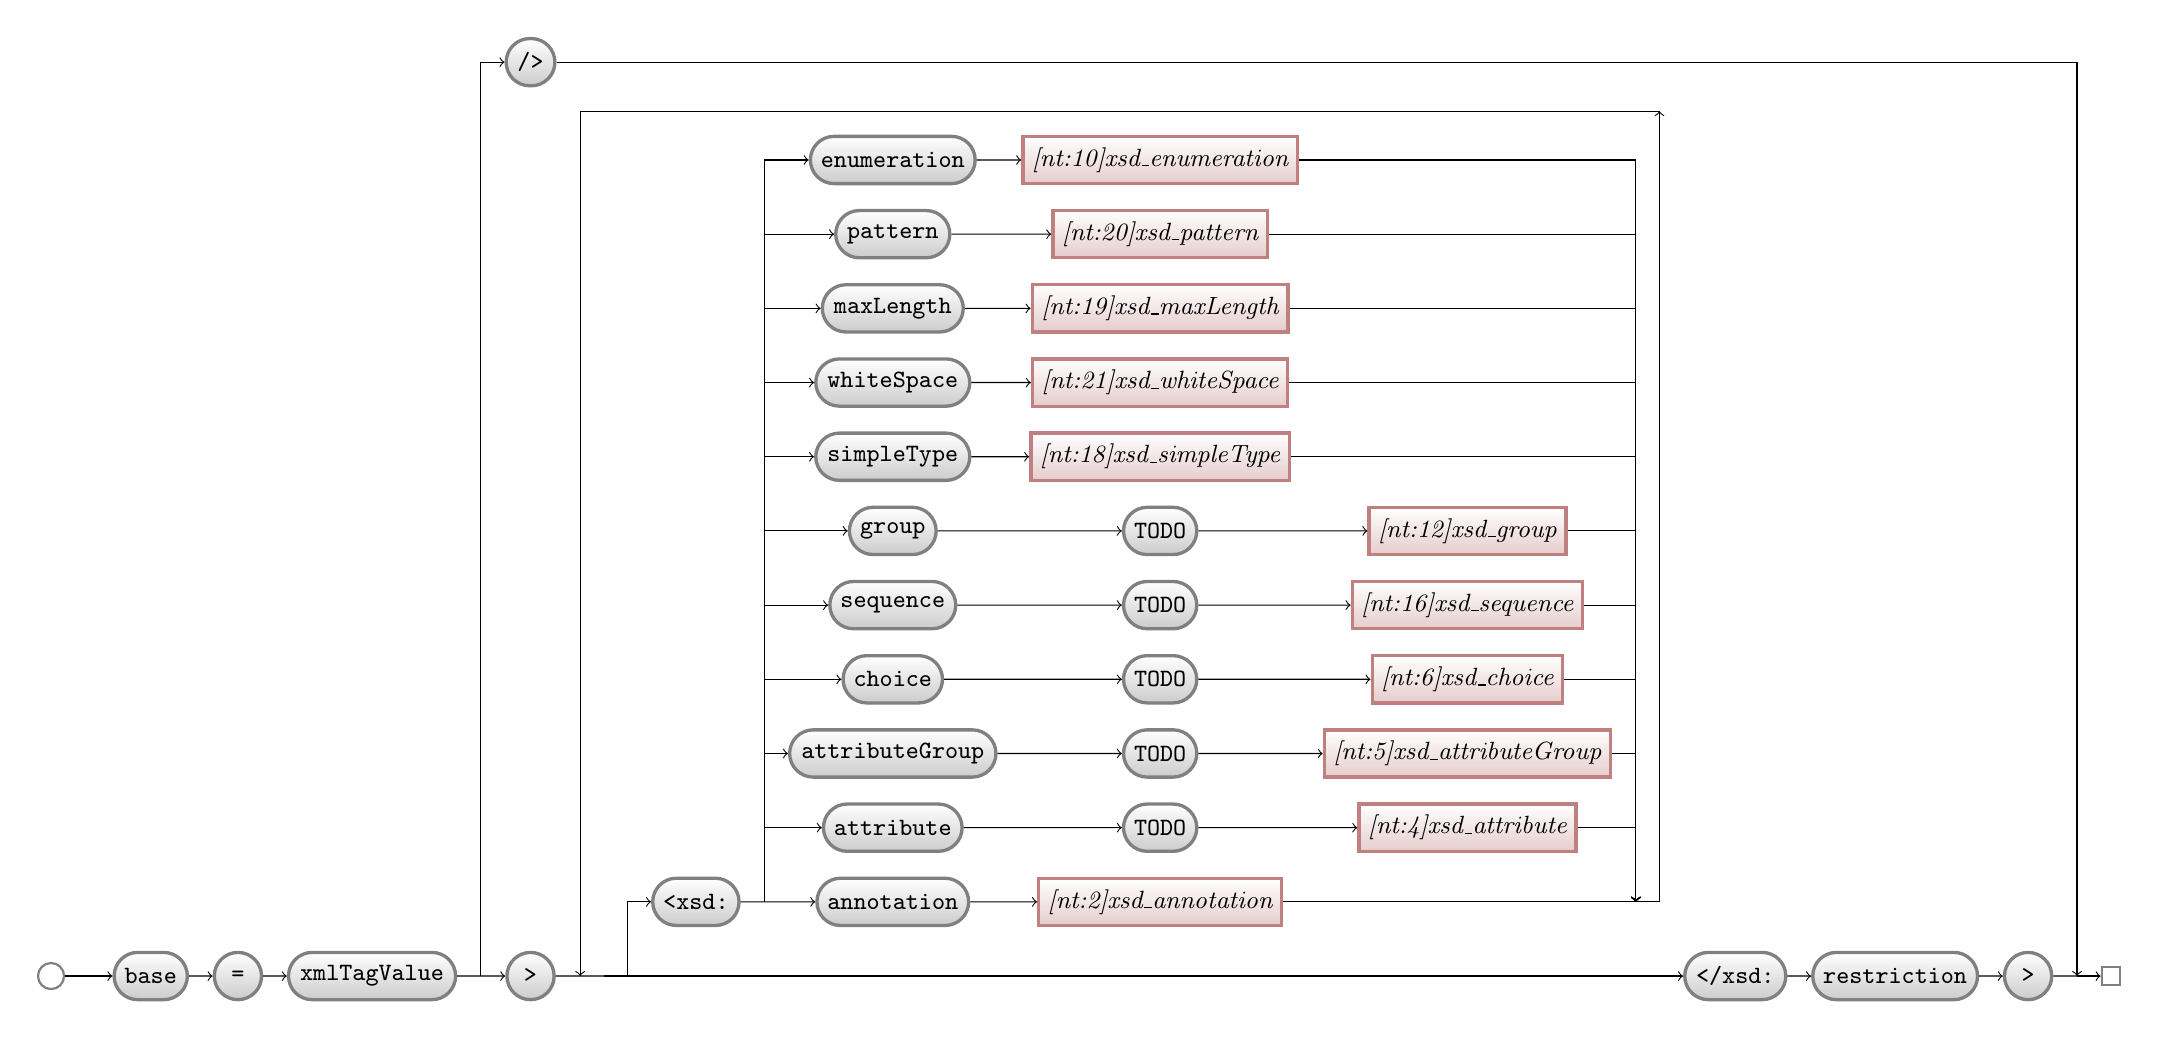
\begin{tikzpicture}
  \matrix[column sep=\ruleMatrixColumnSeparation, row sep=\ruleMatrixRowSeparation] {
    & & & & & & \node (p13-6) [terminal] {/>}; & \\
    & & & & & & & & & & & & & & & & \node (p12-16) [point] {}; & \\
    & & & & & & & & & & & & \node (p11-12) [terminal] {enumeration}; & \node (p11-13) [nonterminal] {\nonTerminalSymbol{xsd\_enumeration}{10}}; & \\
    & & & & & & & & & & & & \node (p10-12) [terminal] {pattern}; & \node (p10-13) [nonterminal] {\nonTerminalSymbol{xsd\_pattern}{20}}; & \\
    & & & & & & & & & & & & \node (p9-12) [terminal] {maxLength}; & \node (p9-13) [nonterminal] {\nonTerminalSymbol{xsd\_maxLength}{19}}; & \\
    & & & & & & & & & & & & \node (p8-12) [terminal] {whiteSpace}; & \node (p8-13) [nonterminal] {\nonTerminalSymbol{xsd\_whiteSpace}{21}}; & \\
    & & & & & & & & & & & & \node (p7-12) [terminal] {simpleType}; & \node (p7-13) [nonterminal] {\nonTerminalSymbol{xsd\_simpleType}{18}}; & \\
    & & & & & & & & & & & & \node (p6-12) [terminal] {group}; & \node (p6-13) [terminal] {TODO}; & \node (p6-14) [nonterminal] {\nonTerminalSymbol{xsd\_group}{12}}; & \\
    & & & & & & & & & & & & \node (p5-12) [terminal] {sequence}; & \node (p5-13) [terminal] {TODO}; & \node (p5-14) [nonterminal] {\nonTerminalSymbol{xsd\_sequence}{16}}; & \\
    & & & & & & & & & & & & \node (p4-12) [terminal] {choice}; & \node (p4-13) [terminal] {TODO}; & \node (p4-14) [nonterminal] {\nonTerminalSymbol{xsd\_choice}{6}}; & \\
    & & & & & & & & & & & & \node (p3-12) [terminal] {attributeGroup}; & \node (p3-13) [terminal] {TODO}; & \node (p3-14) [nonterminal] {\nonTerminalSymbol{xsd\_attributeGroup}{5}}; & \\
    & & & & & & & & & & & & \node (p2-12) [terminal] {attribute}; & \node (p2-13) [terminal] {TODO}; & \node (p2-14) [nonterminal] {\nonTerminalSymbol{xsd\_attribute}{4}}; & \\
    & & & & & & & & & & \node (p1-10) [terminal] {<xsd:}; & \node (p1-11) [point] {}; & \node (p1-12) [terminal] {annotation}; & \node (p1-13) [nonterminal] {\nonTerminalSymbol{xsd\_annotation}{2}}; & & \node (p1-15) [point] {}; & \\
    \node (P0start) [firstPoint] {}; & & \node (p0-2) [terminal] {base}; & \node (p0-3) [terminal] {=}; & \node (p0-4) [terminal] {xmlTagValue}; & \node (p0-5) [point] {}; & \node (p0-6) [terminal] {>}; & \node (p0-7) [point] {}; & \node (p0-8) [point] {}; & \node (p0-9) [point] {}; & & & & & & & & \node (p0-17) [terminal] {</xsd:}; & \node (p0-18) [terminal] {restriction}; & \node (p0-19) [terminal] {>}; & \node (p0-20) [point] {}; & \node (p0-21) [lastPoint] {}; & \\
  };
  \draw[->] (P0start) -- (p0-2) ;
  \draw[->] (p0-2) -- (p0-3) ;
  \draw[->] (p0-3) -- (p0-4) ;
  \draw[->] (p0-4) -- (p0-6) ;
  \draw (p0-6) -- (p0-8) ;
  \draw[->] (p0-9) |- (p1-10) ;
  \draw[->] (p1-10) -- (p1-12) ;
  \draw[->] (p1-12) -- (p1-13) ;
  \draw[->] (p1-11) |- (p2-12) ;
  \draw[->] (p2-12) -- (p2-13) ;
  \draw[->] (p2-13) -- (p2-14) ;
  \draw[->] (p1-11) |- (p3-12) ;
  \draw[->] (p3-12) -- (p3-13) ;
  \draw[->] (p3-13) -- (p3-14) ;
  \draw[->] (p1-11) |- (p4-12) ;
  \draw[->] (p4-12) -- (p4-13) ;
  \draw[->] (p4-13) -- (p4-14) ;
  \draw[->] (p1-11) |- (p5-12) ;
  \draw[->] (p5-12) -- (p5-13) ;
  \draw[->] (p5-13) -- (p5-14) ;
  \draw[->] (p1-11) |- (p6-12) ;
  \draw[->] (p6-12) -- (p6-13) ;
  \draw[->] (p6-13) -- (p6-14) ;
  \draw[->] (p1-11) |- (p7-12) ;
  \draw[->] (p7-12) -- (p7-13) ;
  \draw[->] (p1-11) |- (p8-12) ;
  \draw[->] (p8-12) -- (p8-13) ;
  \draw[->] (p1-11) |- (p9-12) ;
  \draw[->] (p9-12) -- (p9-13) ;
  \draw[->] (p1-11) |- (p10-12) ;
  \draw[->] (p10-12) -- (p10-13) ;
  \draw[->] (p1-11) |- (p11-12) ;
  \draw[->] (p11-12) -- (p11-13) ;
  \draw (p1-13) -- (p1-15) ;
  \draw[->] (p2-14) -| (p1-15) ;
  \draw[->] (p3-14) -| (p1-15) ;
  \draw[->] (p4-14) -| (p1-15) ;
  \draw[->] (p5-14) -| (p1-15) ;
  \draw[->] (p6-14) -| (p1-15) ;
  \draw[->] (p7-13) -| (p1-15) ;
  \draw[->] (p8-13) -| (p1-15) ;
  \draw[->] (p9-13) -| (p1-15) ;
  \draw[->] (p10-13) -| (p1-15) ;
  \draw[->] (p11-13) -| (p1-15) ;
  \draw[->] (p12-16) -| (p0-7) ;
  \draw[->] (p1-15) -| (p12-16) ;
  \draw[->] (p0-8) -- (p0-17) ;
  \draw[->] (p0-17) -- (p0-18) ;
  \draw[->] (p0-18) -- (p0-19) ;
  \draw[->] (p0-5) |- (p13-6) ;
  \draw (p0-19) -- (p0-20) ;
  \draw[->] (p13-6) -| (p0-20) ;
  \draw[->] (p0-20) -- (p0-21) ;
\end{tikzpicture}

\nonTerminalSection{xsd\_schema}{15}

\ruleSubsection{arxmlmetaparser\_syntax}{arxmlmetaparser\_syntax}{753}

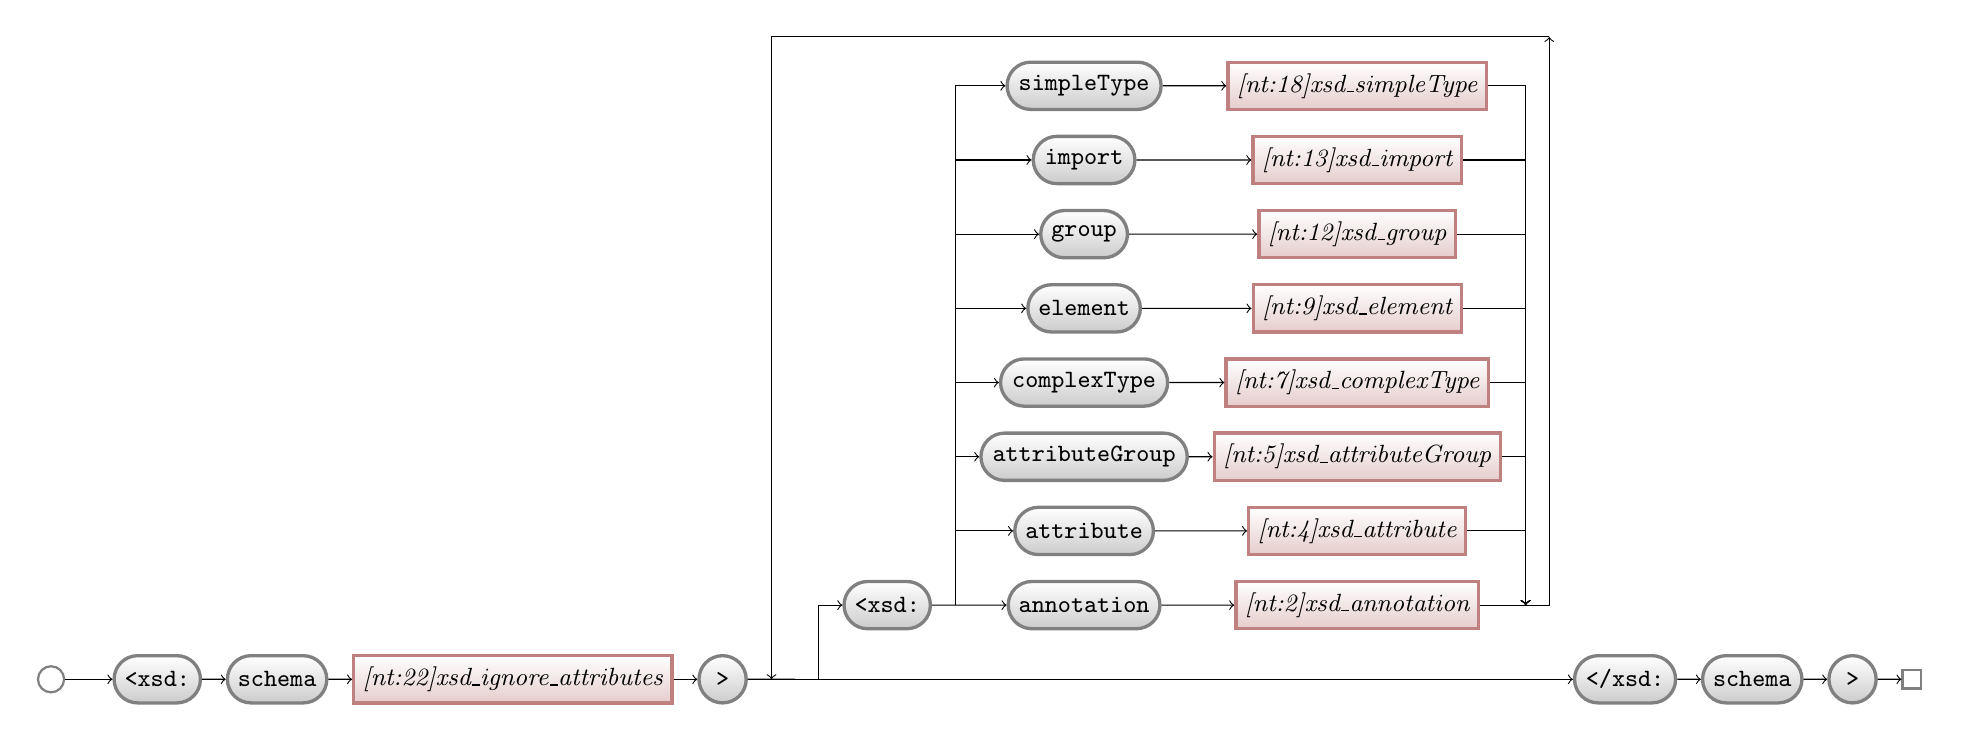
\begin{tikzpicture}
  \matrix[column sep=\ruleMatrixColumnSeparation, row sep=\ruleMatrixRowSeparation] {
    & & & & & & & & & & & & & & \node (p9-14) [point] {}; & \\
    & & & & & & & & & & & \node (p8-11) [terminal] {simpleType}; & \node (p8-12) [nonterminal] {\nonTerminalSymbol{xsd\_simpleType}{18}}; & \\
    & & & & & & & & & & & \node (p7-11) [terminal] {import}; & \node (p7-12) [nonterminal] {\nonTerminalSymbol{xsd\_import}{13}}; & \\
    & & & & & & & & & & & \node (p6-11) [terminal] {group}; & \node (p6-12) [nonterminal] {\nonTerminalSymbol{xsd\_group}{12}}; & \\
    & & & & & & & & & & & \node (p5-11) [terminal] {element}; & \node (p5-12) [nonterminal] {\nonTerminalSymbol{xsd\_element}{9}}; & \\
    & & & & & & & & & & & \node (p4-11) [terminal] {complexType}; & \node (p4-12) [nonterminal] {\nonTerminalSymbol{xsd\_complexType}{7}}; & \\
    & & & & & & & & & & & \node (p3-11) [terminal] {attributeGroup}; & \node (p3-12) [nonterminal] {\nonTerminalSymbol{xsd\_attributeGroup}{5}}; & \\
    & & & & & & & & & & & \node (p2-11) [terminal] {attribute}; & \node (p2-12) [nonterminal] {\nonTerminalSymbol{xsd\_attribute}{4}}; & \\
    & & & & & & & & & \node (p1-9) [terminal] {<xsd:}; & \node (p1-10) [point] {}; & \node (p1-11) [terminal] {annotation}; & \node (p1-12) [nonterminal] {\nonTerminalSymbol{xsd\_annotation}{2}}; & \node (p1-13) [point] {}; & \\
    \node (P0start) [firstPoint] {}; & & \node (p0-2) [terminal] {<xsd:}; & \node (p0-3) [terminal] {schema}; & \node (p0-4) [nonterminal] {\nonTerminalSymbol{xsd\_ignore\_attributes}{22}}; & \node (p0-5) [terminal] {>}; & \node (p0-6) [point] {}; & \node (p0-7) [point] {}; & \node (p0-8) [point] {}; & & & & & & & \node (p0-15) [terminal] {</xsd:}; & \node (p0-16) [terminal] {schema}; & \node (p0-17) [terminal] {>}; & \node (p0-18) [lastPoint] {}; & \\
  };
  \draw[->] (P0start) -- (p0-2) ;
  \draw[->] (p0-2) -- (p0-3) ;
  \draw[->] (p0-3) -- (p0-4) ;
  \draw[->] (p0-4) -- (p0-5) ;
  \draw (p0-5) -- (p0-7) ;
  \draw[->] (p0-8) |- (p1-9) ;
  \draw[->] (p1-9) -- (p1-11) ;
  \draw[->] (p1-11) -- (p1-12) ;
  \draw[->] (p1-10) |- (p2-11) ;
  \draw[->] (p2-11) -- (p2-12) ;
  \draw[->] (p1-10) |- (p3-11) ;
  \draw[->] (p3-11) -- (p3-12) ;
  \draw[->] (p1-10) |- (p4-11) ;
  \draw[->] (p4-11) -- (p4-12) ;
  \draw[->] (p1-10) |- (p5-11) ;
  \draw[->] (p5-11) -- (p5-12) ;
  \draw[->] (p1-10) |- (p6-11) ;
  \draw[->] (p6-11) -- (p6-12) ;
  \draw[->] (p1-10) |- (p7-11) ;
  \draw[->] (p7-11) -- (p7-12) ;
  \draw[->] (p1-10) |- (p8-11) ;
  \draw[->] (p8-11) -- (p8-12) ;
  \draw (p1-12) -- (p1-13) ;
  \draw[->] (p2-12) -| (p1-13) ;
  \draw[->] (p3-12) -| (p1-13) ;
  \draw[->] (p4-12) -| (p1-13) ;
  \draw[->] (p5-12) -| (p1-13) ;
  \draw[->] (p6-12) -| (p1-13) ;
  \draw[->] (p7-12) -| (p1-13) ;
  \draw[->] (p8-12) -| (p1-13) ;
  \draw[->] (p9-14) -| (p0-6) ;
  \draw[->] (p1-13) -| (p9-14) ;
  \draw[->] (p0-7) -- (p0-15) ;
  \draw[->] (p0-15) -- (p0-16) ;
  \draw[->] (p0-16) -- (p0-17) ;
  \draw[->] (p0-17) -- (p0-18) ;
\end{tikzpicture}

\nonTerminalSection{xsd\_sequence}{16}

\ruleSubsection{arxmlmetaparser\_syntax}{arxmlmetaparser\_syntax}{810}

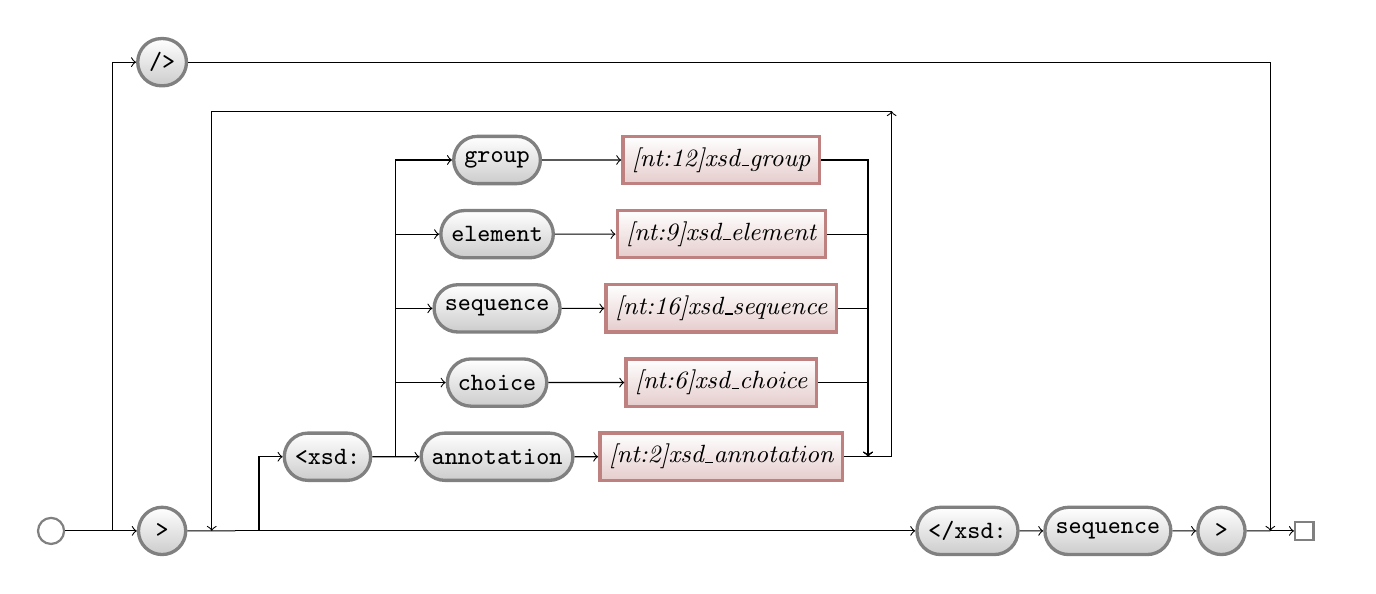
\begin{tikzpicture}
  \matrix[column sep=\ruleMatrixColumnSeparation, row sep=\ruleMatrixRowSeparation] {
    & & & \node (p7-3) [terminal] {/>}; & \\
    & & & & & & & & & & & & \node (p6-12) [point] {}; & \\
    & & & & & & & & & \node (p5-9) [terminal] {group}; & \node (p5-10) [nonterminal] {\nonTerminalSymbol{xsd\_group}{12}}; & \\
    & & & & & & & & & \node (p4-9) [terminal] {element}; & \node (p4-10) [nonterminal] {\nonTerminalSymbol{xsd\_element}{9}}; & \\
    & & & & & & & & & \node (p3-9) [terminal] {sequence}; & \node (p3-10) [nonterminal] {\nonTerminalSymbol{xsd\_sequence}{16}}; & \\
    & & & & & & & & & \node (p2-9) [terminal] {choice}; & \node (p2-10) [nonterminal] {\nonTerminalSymbol{xsd\_choice}{6}}; & \\
    & & & & & & & \node (p1-7) [terminal] {<xsd:}; & \node (p1-8) [point] {}; & \node (p1-9) [terminal] {annotation}; & \node (p1-10) [nonterminal] {\nonTerminalSymbol{xsd\_annotation}{2}}; & \node (p1-11) [point] {}; & \\
    \node (P0start) [firstPoint] {}; & & \node (p0-2) [point] {}; & \node (p0-3) [terminal] {>}; & \node (p0-4) [point] {}; & \node (p0-5) [point] {}; & \node (p0-6) [point] {}; & & & & & & & \node (p0-13) [terminal] {</xsd:}; & \node (p0-14) [terminal] {sequence}; & \node (p0-15) [terminal] {>}; & \node (p0-16) [point] {}; & \node (p0-17) [lastPoint] {}; & \\
  };
  \draw[->] (P0start) -- (p0-3) ;
  \draw (p0-3) -- (p0-5) ;
  \draw[->] (p0-6) |- (p1-7) ;
  \draw[->] (p1-7) -- (p1-9) ;
  \draw[->] (p1-9) -- (p1-10) ;
  \draw[->] (p1-8) |- (p2-9) ;
  \draw[->] (p2-9) -- (p2-10) ;
  \draw[->] (p1-8) |- (p3-9) ;
  \draw[->] (p3-9) -- (p3-10) ;
  \draw[->] (p1-8) |- (p4-9) ;
  \draw[->] (p4-9) -- (p4-10) ;
  \draw[->] (p1-8) |- (p5-9) ;
  \draw[->] (p5-9) -- (p5-10) ;
  \draw (p1-10) -- (p1-11) ;
  \draw[->] (p2-10) -| (p1-11) ;
  \draw[->] (p3-10) -| (p1-11) ;
  \draw[->] (p4-10) -| (p1-11) ;
  \draw[->] (p5-10) -| (p1-11) ;
  \draw[->] (p6-12) -| (p0-4) ;
  \draw[->] (p1-11) -| (p6-12) ;
  \draw[->] (p0-5) -- (p0-13) ;
  \draw[->] (p0-13) -- (p0-14) ;
  \draw[->] (p0-14) -- (p0-15) ;
  \draw[->] (p0-2) |- (p7-3) ;
  \draw (p0-15) -- (p0-16) ;
  \draw[->] (p7-3) -| (p0-16) ;
  \draw[->] (p0-16) -- (p0-17) ;
\end{tikzpicture}

\nonTerminalSection{xsd\_simpleContent}{17}

\ruleSubsection{arxmlmetaparser\_syntax}{arxmlmetaparser\_syntax}{841}

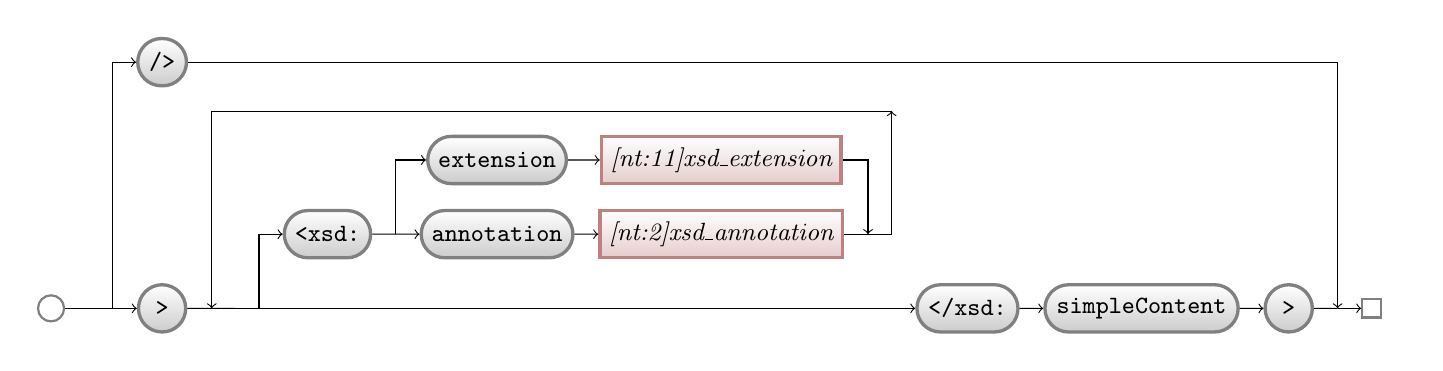
\begin{tikzpicture}
  \matrix[column sep=\ruleMatrixColumnSeparation, row sep=\ruleMatrixRowSeparation] {
    & & & \node (p4-3) [terminal] {/>}; & \\
    & & & & & & & & & & & & \node (p3-12) [point] {}; & \\
    & & & & & & & & & \node (p2-9) [terminal] {extension}; & \node (p2-10) [nonterminal] {\nonTerminalSymbol{xsd\_extension}{11}}; & \\
    & & & & & & & \node (p1-7) [terminal] {<xsd:}; & \node (p1-8) [point] {}; & \node (p1-9) [terminal] {annotation}; & \node (p1-10) [nonterminal] {\nonTerminalSymbol{xsd\_annotation}{2}}; & \node (p1-11) [point] {}; & \\
    \node (P0start) [firstPoint] {}; & & \node (p0-2) [point] {}; & \node (p0-3) [terminal] {>}; & \node (p0-4) [point] {}; & \node (p0-5) [point] {}; & \node (p0-6) [point] {}; & & & & & & & \node (p0-13) [terminal] {</xsd:}; & \node (p0-14) [terminal] {simpleContent}; & \node (p0-15) [terminal] {>}; & \node (p0-16) [point] {}; & \node (p0-17) [lastPoint] {}; & \\
  };
  \draw[->] (P0start) -- (p0-3) ;
  \draw (p0-3) -- (p0-5) ;
  \draw[->] (p0-6) |- (p1-7) ;
  \draw[->] (p1-7) -- (p1-9) ;
  \draw[->] (p1-9) -- (p1-10) ;
  \draw[->] (p1-8) |- (p2-9) ;
  \draw[->] (p2-9) -- (p2-10) ;
  \draw (p1-10) -- (p1-11) ;
  \draw[->] (p2-10) -| (p1-11) ;
  \draw[->] (p3-12) -| (p0-4) ;
  \draw[->] (p1-11) -| (p3-12) ;
  \draw[->] (p0-5) -- (p0-13) ;
  \draw[->] (p0-13) -- (p0-14) ;
  \draw[->] (p0-14) -- (p0-15) ;
  \draw[->] (p0-2) |- (p4-3) ;
  \draw (p0-15) -- (p0-16) ;
  \draw[->] (p4-3) -| (p0-16) ;
  \draw[->] (p0-16) -- (p0-17) ;
\end{tikzpicture}

\nonTerminalSection{xsd\_simpleType}{18}

\ruleSubsection{arxmlmetaparser\_syntax}{arxmlmetaparser\_syntax}{876}

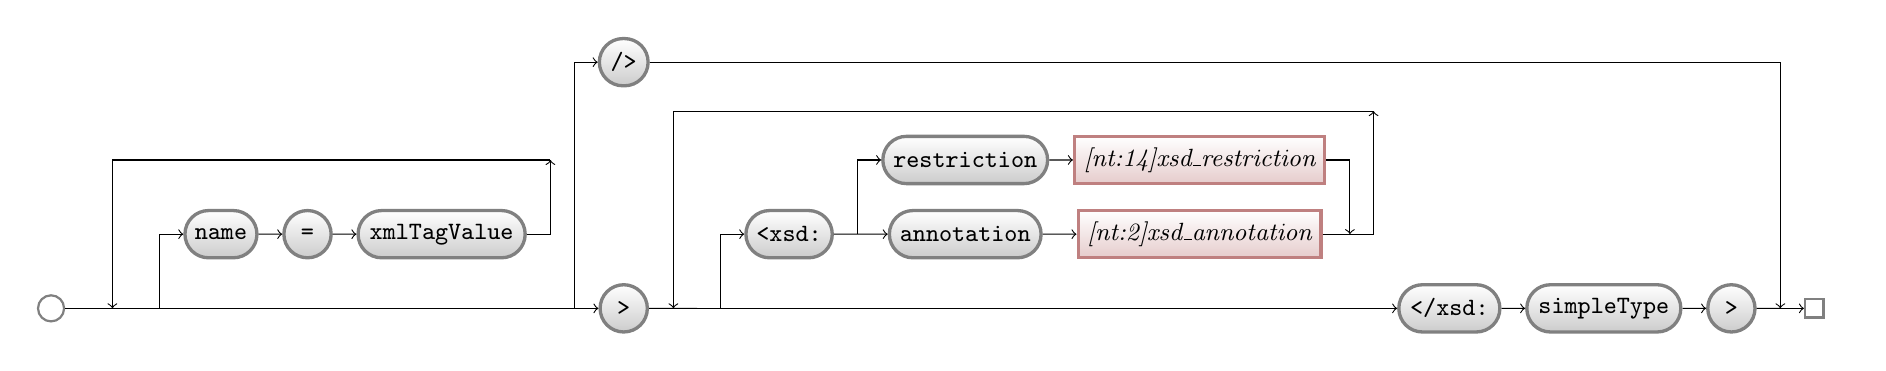
\begin{tikzpicture}
  \matrix[column sep=\ruleMatrixColumnSeparation, row sep=\ruleMatrixRowSeparation] {
    & & & & & & & & & & \node (p4-10) [terminal] {/>}; & \\
    & & & & & & & & & & & & & & & & & & & \node (p3-19) [point] {}; & \\
    & & & & & & & & \node (p2-8) [point] {}; & & & & & & & & \node (p2-16) [terminal] {restriction}; & \node (p2-17) [nonterminal] {\nonTerminalSymbol{xsd\_restriction}{14}}; & \\
    & & & & & \node (p1-5) [terminal] {name}; & \node (p1-6) [terminal] {=}; & \node (p1-7) [terminal] {xmlTagValue}; & & & & & & & \node (p1-14) [terminal] {<xsd:}; & \node (p1-15) [point] {}; & \node (p1-16) [terminal] {annotation}; & \node (p1-17) [nonterminal] {\nonTerminalSymbol{xsd\_annotation}{2}}; & \node (p1-18) [point] {}; & \\
    \node (P0start) [firstPoint] {}; & & \node (p0-2) [point] {}; & \node (p0-3) [point] {}; & \node (p0-4) [point] {}; & & & & & \node (p0-9) [point] {}; & \node (p0-10) [terminal] {>}; & \node (p0-11) [point] {}; & \node (p0-12) [point] {}; & \node (p0-13) [point] {}; & & & & & & & \node (p0-20) [terminal] {</xsd:}; & \node (p0-21) [terminal] {simpleType}; & \node (p0-22) [terminal] {>}; & \node (p0-23) [point] {}; & \node (p0-24) [lastPoint] {}; & \\
  };
  \draw (P0start) -- (p0-3) ;
  \draw[->] (p0-4) |- (p1-5) ;
  \draw[->] (p1-5) -- (p1-6) ;
  \draw[->] (p1-6) -- (p1-7) ;
  \draw[->] (p2-8) -| (p0-2) ;
  \draw[->] (p1-7) -| (p2-8) ;
  \draw[->] (p0-3) -- (p0-10) ;
  \draw (p0-10) -- (p0-12) ;
  \draw[->] (p0-13) |- (p1-14) ;
  \draw[->] (p1-14) -- (p1-16) ;
  \draw[->] (p1-16) -- (p1-17) ;
  \draw[->] (p1-15) |- (p2-16) ;
  \draw[->] (p2-16) -- (p2-17) ;
  \draw (p1-17) -- (p1-18) ;
  \draw[->] (p2-17) -| (p1-18) ;
  \draw[->] (p3-19) -| (p0-11) ;
  \draw[->] (p1-18) -| (p3-19) ;
  \draw[->] (p0-12) -- (p0-20) ;
  \draw[->] (p0-20) -- (p0-21) ;
  \draw[->] (p0-21) -- (p0-22) ;
  \draw[->] (p0-9) |- (p4-10) ;
  \draw (p0-22) -- (p0-23) ;
  \draw[->] (p4-10) -| (p0-23) ;
  \draw[->] (p0-23) -- (p0-24) ;
\end{tikzpicture}

\nonTerminalSection{xsd\_whiteSpace}{21}

\ruleSubsection{arxmlmetaparser\_syntax}{arxmlmetaparser\_syntax}{991}

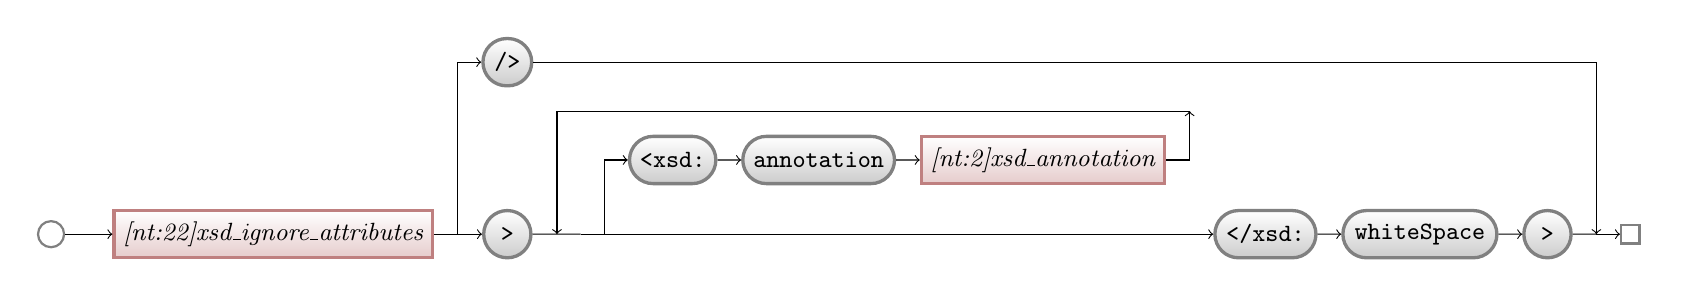
\begin{tikzpicture}
  \matrix[column sep=\ruleMatrixColumnSeparation, row sep=\ruleMatrixRowSeparation] {
    & & & & \node (p3-4) [terminal] {/>}; & \\
    & & & & & & & & & & & \node (p2-11) [point] {}; & \\
    & & & & & & & & \node (p1-8) [terminal] {<xsd:}; & \node (p1-9) [terminal] {annotation}; & \node (p1-10) [nonterminal] {\nonTerminalSymbol{xsd\_annotation}{2}}; & \\
    \node (P0start) [firstPoint] {}; & & \node (p0-2) [nonterminal] {\nonTerminalSymbol{xsd\_ignore\_attributes}{22}}; & \node (p0-3) [point] {}; & \node (p0-4) [terminal] {>}; & \node (p0-5) [point] {}; & \node (p0-6) [point] {}; & \node (p0-7) [point] {}; & & & & & \node (p0-12) [terminal] {</xsd:}; & \node (p0-13) [terminal] {whiteSpace}; & \node (p0-14) [terminal] {>}; & \node (p0-15) [point] {}; & \node (p0-16) [lastPoint] {}; & \\
  };
  \draw[->] (P0start) -- (p0-2) ;
  \draw[->] (p0-2) -- (p0-4) ;
  \draw (p0-4) -- (p0-6) ;
  \draw[->] (p0-7) |- (p1-8) ;
  \draw[->] (p1-8) -- (p1-9) ;
  \draw[->] (p1-9) -- (p1-10) ;
  \draw[->] (p2-11) -| (p0-5) ;
  \draw[->] (p1-10) -| (p2-11) ;
  \draw[->] (p0-6) -- (p0-12) ;
  \draw[->] (p0-12) -- (p0-13) ;
  \draw[->] (p0-13) -- (p0-14) ;
  \draw[->] (p0-3) |- (p3-4) ;
  \draw (p0-14) -- (p0-15) ;
  \draw[->] (p3-4) -| (p0-15) ;
  \draw[->] (p0-15) -- (p0-16) ;
\end{tikzpicture}



\end{document}
